% arXiv preprint — The Synthetic Economy
\documentclass[11pt]{article}

% ── Packages ──────────────────────────────────────────────────────────
\usepackage[margin=1in]{geometry}
\usepackage[T1]{fontenc}
\usepackage{amsmath,amssymb}
\usepackage{graphicx}
\usepackage{booktabs}
\usepackage{multirow}
\usepackage{balance}
\usepackage{hyperref}
\hypersetup{colorlinks=true, linkcolor=blue, citecolor=blue, urlcolor=blue}
\usepackage{xcolor}
\usepackage{enumitem}
\usepackage[expansion=false]{microtype}
\usepackage{subcaption}
\sloppy

% ── arXiv metadata ────────────────────────────────────────────────────
\newcommand{\paperversion}{v3}
\newcommand{\paperyear}{2026}

\title{The Synthetic Economy:\\
Can Small Language Models Generate\\
Research-Grade Economic Microdata?%
\thanks{This work was produced with a total API budget of \$0.08 using four low-cost hosted language models. Code and data: \url{https://github.com/mnnekrashevich/synth-eco}}}

\author{
  Mikhail N. Nekrashevich\\
  Department of Information Systems and Digital Technologies,\\
  Faculty of Mathematics and Information Technologies,\\
  Orel State University named after I.S.\ Turgenev\\
  Orel, Russia\\
  \texttt{mn.nekrashevich@yandex.ru}\\
  ORCID: 0009-0005-1808-8906
}

\date{}

\begin{document}
\maketitle

% ══════════════════════════════════════════════════════════════════════
% ABSTRACT
% ══════════════════════════════════════════════════════════════════════
\begin{abstract}
Synthetic microdata are increasingly proposed as a privacy-preserving substitute for confidential survey data, yet most generative approaches require substantial compute and access to real training records.
We investigate whether small, low-cost language models---Ling 3.0 Flash, DeepSeek~V4 Flash, Solar Pro~4, and Qwen~3.7~Flash, priced at under \$0.03 each---can generate research-grade synthetic economic microdata from a text prompt alone, with no fine-tuning and no access to real records.
Using public aggregated statistics from the U.S.\ Current Population Survey as ground truth, we generate 800 synthetic household records per model per condition (2{,}400 per model) across three prompt conditions (minimal, structural, priors) and evaluate them along four dimensions: statistical fidelity, downstream econometric utility, internal consistency, and diversity.
We find that the models reproduce conditional economic structure remarkably well---education--income gradients within 4.7--11.6\% mean absolute relative error, Mincer wage regressions with $R^2 = 0.86$--0.90, and near-perfect internal consistency between employment, hours, and income---but systematically distort unconditional marginals, overstating the employment rate (62--83\% vs.\ 63\% reference) and the share of advanced degrees.
A three-condition prompt ablation isolates the contribution of the models' \emph{latent} economic knowledge from \emph{explicit} priors supplied in the prompt, revealing that explicit priors substantially improve income fidelity (MARE reduction of 40--53\%) while having limited effect on econometric utility ($R^2$ changes $< 0.04$).
Compared with two non-LLM baselines (uniform and marginal sampling), the LLMs' unique value lies in their joint structure ($R^2 \geq 0.86$), not their marginals---a marginal sampler achieves MARE of 2.9\% but $R^2$ of only 0.23.
We then demonstrate that the paper's recommended remedy works: a single post-stratification step that reweights records to match the public education distribution drives the education-distribution total variation distance to zero while leaving the Mincer $R^2$ essentially unchanged (within $\pm 0.02$), confirming that the LLMs' joint structure survives marginal calibration.
Cross-seed analysis demonstrates high reproducibility (coefficient of variation $< 3.4\%$ for $R^2$), and Wasserstein-distance analysis reveals that the synthetic income distributions are within 15--21\% of the reference in normalized earth-mover distance.
Our results establish that small language models can serve as cheap, zero-shot generators of structurally coherent economic microdata, and that a lightweight, fully public calibration step renders them fit for research use---at a total cost of under \$0.10.
\end{abstract}

\medskip
\noindent\textbf{Keywords:} synthetic data, large language models, economic microdata, Current Population Survey, Mincer regression, data fidelity, prompt ablation, reproducibility

% ══════════════════════════════════════════════════════════════════════
% 1. INTRODUCTION
% ══════════════════════════════════════════════════════════════════════
\section{Introduction}
\label{sec:introduction}

Confidential survey microdata---such as the U.S.\ Current Population Survey (CPS)---are the empirical backbone of labor economics, yet their release is tightly restricted to protect respondent privacy.
Synthetic data generation has emerged as a leading strategy to reconcile the demand for granular microdata with privacy constraints~\cite{seedat2024curatedllm}.
Traditional generative approaches (GANs, VAEs, diffusion models) require training on the real data they aim to replace, which both demands substantial compute and inherits the very privacy risks they seek to avoid.

Large language models (LLMs) offer a qualitatively different route: because they encode broad world knowledge, they can in principle generate plausible microdata \emph{zero-shot}, from a text description alone, without ever seeing a real record~\cite{borisov2023great,fang2024llmtabular}.
This would make synthetic data generation dramatically cheaper and, by construction, free of direct record-level leakage.
However, prior work has largely focused on large, expensive frontier models (e.g., GPT-4) and on fine-tuned or curated pipelines~\cite{seedat2024curatedllm}.
Whether a \emph{small}, \emph{cheap} model can produce research-grade economic microdata from a prompt alone remains an open and practically important question.

\subsection{Motivation}

The practical stakes are concrete.
Researchers in developing countries often lack access to confidential microdata, yet must calibrate policy simulations against realistic population distributions.
Educators teaching econometrics need realistic datasets for lab exercises but cannot distribute real CPS records.
Data scientists prototyping ML pipelines for credit scoring or labor-market analysis need structurally coherent synthetic populations for unit testing.
In each case, the desideratum is not perfect statistical fidelity, but \emph{conditional structure}: the education--income gradient, the employment--hours--income consistency, and the concave age--earnings profile that makes a synthetic population behave like a real one in regression analysis.

This paper addresses that question with a deliberately minimal setup: four low-cost hosted models (Ling 3.0 Flash, DeepSeek V4 Flash, Solar Pro 4, and Qwen 3.7 Flash, each under \$0.03 for the entire study), a single text prompt encoding basic economic priors, and no fine-tuning, no real training data, and no curation.
We generate 800 synthetic household records per model and benchmark them against public aggregated CPS statistics.
Our contributions are:

\begin{enumerate}[leftmargin=*, itemsep=2pt]
  \item A reproducible, near-zero-cost protocol for generating synthetic economic microdata from small LLMs, with total API spend under \$0.08 across four models.
  \item A four-dimensional evaluation (fidelity, downstream utility, consistency, diversity) against public CPS aggregates, augmented with Wasserstein distances and cross-model Jensen--Shannon divergence, with bootstrap confidence intervals and two non-LLM baselines (uniform and marginal sampling) to contextualize the results.
  \item A three-condition prompt ablation (minimal, structural, priors) across all four models that isolates the contribution of the models' \emph{latent} economic knowledge from the \emph{explicit} priors supplied in the prompt.
  \item Cross-seed reproducibility analysis demonstrating that the Mincer $R^2$ is stable across random seeds (coefficient of variation $< 3.4\%$), establishing the reliability of the generation protocol.
  \item Evidence that small LLMs capture \emph{conditional} economic structure (education$\rightarrow$income, employment$\rightarrow$hours) far better than \emph{unconditional} marginals (employment rate, education distribution), identifying precisely where post-hoc correction is needed.
  \item A concrete demonstration that the recommended remedy works: post-stratifying the synthetic records to match the public education distribution drives the education-distribution TVD to zero while preserving the Mincer $R^2$ (within $\pm 0.02$), validating the proposed generate--validate--calibrate--verify recipe end to end.
\end{enumerate}

The remainder of this paper is organized as follows.
Section~\ref{sec:related} reviews related work.
Section~\ref{sec:method} describes our generation and evaluation methodology.
Section~\ref{sec:results} presents results.
Section~\ref{sec:discussion} discusses implications and limitations.
Section~\ref{sec:conclusion} concludes.

% ══════════════════════════════════════════════════════════════════════
% 2. RELATED WORK
% ══════════════════════════════════════════════════════════════════════
\section{Related Work}
\label{sec:related}

\subsection{Classical Synthetic Data Generation}

Before LLMs, synthetic tabular data was generated by statistical and deep generative models.
Copula-based methods, as implemented in the Synthetic Data Vault~\cite{patki2016synthpop}, model the joint distribution of features and sample from it.
GAN-based approaches such as CTGAN~\cite{xu2019ctgan} and its variational counterpart TVAE~\cite{xu2019tve} learn to generate realistic rows from training data.
In the economics domain, the \texttt{synthpop} package~\cite{nowok2016synthpop} synthesizes population microdata from real survey records.
All of these methods share a common requirement: they must be \emph{trained on the real data} they aim to replace, which both demands compute and inherits the privacy risks of the source data.
Differential-privacy-aware generators~\cite{tao2024benchmarking} mitigate the latter but typically at a substantial cost to utility.

\subsection{LLM-Based Tabular Data Generation}

The use of language models to generate tabular data has grown rapidly.
GReaT~\cite{borisov2023great} established the core pipeline of serializing tabular rows as text and fine-tuning an LLM to generate new rows, demonstrating that language models can be realistic tabular data generators.
Curated LLM~\cite{seedat2024curatedllm} showed that in low-data regimes, a frozen LLM prompted with feature descriptions and a few examples can augment datasets, and that a principled curation mechanism substantially improves downstream utility.
Fang et al.~\cite{fang2024llmtabular} survey the broader landscape of LLM methods for tabular prediction, generation, and understanding.
More recent work has explored zero-shot generation from structured prompts~\cite{braun2025synthetic}, privacy-preserving fine-tuning~\cite{chen2025privsynth}, and the use of smaller, cheaper models for data augmentation~\cite{lee2025smallllm}.
Several 2025--2026 studies have specifically examined the fidelity of LLM-generated tabular data, finding that instruction-tuned models can produce realistic distributions when provided with detailed schema descriptions and marginal constraints~\cite{mousavi2025llmtable,gupta2025syntheticllm}.
Concurrent 2026 work has begun to characterize the systematic biases of zero-shot LLM generators---in particular, their tendency to over-represent salient but rare categories and to distort unconditional base rates---and to propose calibration as a remedy~\cite{zhang2026llmcalib,liu2026syntheticbias}.
Our calibration demonstration (Section~\ref{sec:calibration}) provides direct empirical evidence for this proposed remedy in the economic-microdata setting.

\subsection{LLMs for Economic and Social Science Data}

A smaller but growing literature applies LLMs specifically to economic data generation.
Ante et al.~\cite{ante2025llmeconomics} use LLMs to generate synthetic economic indicators for nowcasting.
Huang et al.~\cite{huang2025llmsurvey} survey the use of LLMs in social science research, noting their potential for generating training data.
However, no prior study systematically evaluates whether small, low-cost LLMs can reproduce the \emph{econometric structure} of a real household survey---specifically, whether a Mincer wage regression fit on synthetic data recovers canonical economic parameters.

\subsection{Gap}

Two features distinguish our work from this prior art.
First, prior LLM generators either fine-tune the model~\cite{borisov2023great} or provide in-context examples and curation~\cite{seedat2024curatedllm}; we use a \emph{pure zero-shot} prompt with no examples and no curation, isolating the model's prior knowledge.
Second, prior work emphasizes large frontier models; we deliberately use small, sub-\$0.03 models to test the practical floor of what is achievable.
To our knowledge, no prior study evaluates whether small LLMs can reproduce the \emph{econometric structure} of a real survey---specifically, whether a Mincer wage regression fit on synthetic data recovers canonical economic parameters---across multiple models under controlled prompt ablation.
Crucially, we also compare against simple non-LLM baselines (uniform and marginal sampling), which prior LLM tabular-generation papers rarely do, and we run a prompt ablation to separate latent knowledge from instructed priors.
Finally, we provide cross-seed reproducibility analysis and Wasserstein-distance metrics to complement standard MARE and $R^2$ measures.

% ══════════════════════════════════════════════════════════════════════
% 3. METHODOLOGY
% ══════════════════════════════════════════════════════════════════════
\section{Methodology}
\label{sec:method}

\subsection{Problem Formulation}

We study the following problem: given a text prompt describing a population survey schema and (optionally) aggregated statistics, can a small language model generate a set of synthetic records $\tilde{X} = \{\tilde{x}_1, \ldots, \tilde{x}_n\}$ whose statistical properties approximate those of a real population $X$?
We evaluate approximation along four dimensions: (i)~marginal fidelity---how close are the synthetic univariate distributions to the reference?; (ii)~conditional fidelity---how well do the synthetic data preserve relationships between variables?; (iii)~downstream utility---can a researcher obtain similar econometric estimates from synthetic data as from real data?; and (iv)~consistency---are the synthetic records internally logically coherent?

Our evaluation uses public aggregated statistics from the U.S.\ Current Population Survey~\cite{bls2024earnings,bls2024unemployment,census2024attainment} as the ground-truth reference $X$. We do not have access to the actual CPS microdata; this is by design, as our protocol must be reproducible without restricted data access.

\subsection{Models}

We evaluate four small, low-cost hosted language models served via the OpenRouter API: Ling 3.0 Flash (\$0.021/M input, \$0.063/M output), DeepSeek V4 Flash (\$0.030/M, \$0.160/M), Solar Pro 4 (\$0.030/M, \$0.120/M), and Qwen 3.7 Flash (\$0.025/M, \$0.080/M).
All four models were released or updated in mid-2026 and represent the current state of small, affordable language models.
Reasoning was disabled (``effort: none'') where supported to reduce cost and ensure clean JSON output.
No real records, examples, or in-context demonstrations were provided.
The total API cost across all four models and all conditions was under \$0.08.

\subsection{Data Generation and Prompt Ablation}

To separate the models' \emph{latent} economic knowledge from the \emph{explicit} priors we supply, we run a three-condition prompt ablation:
\begin{itemize}[leftmargin=*, itemsep=1pt]
  \item \textbf{Minimal}: the prompt specifies only the field schema (age, gender, education, income, employed, hours, marital status, children, state), with no economic guidance.
  \item \textbf{Structural}: adds logical consistency constraints---employed people work positive hours, the non-employed earn zero income, and income follows an age lifecycle---but no target values.
  \item \textbf{Priors}: additionally supplies explicit target values (median income by education, education distribution), matching the original protocol.
\end{itemize}
The full prompts are reproduced in Appendix~\ref{app:prompts}.

Each API call requested a JSON array of 20 records.
We generated 400 records per seed across two seeds ($42$, $2024$), yielding 800 records per model per condition.
Each record contains nine fields: \texttt{age} (18--85), \texttt{gender}, \texttt{education} (high\_school, some\_college, bachelors, masters, phd), \texttt{income} (annual USD), \texttt{employed} (boolean), \texttt{hours\_worked} (0--80), \texttt{marital\_status}, \texttt{children} (0--6), and \texttt{state} (two-letter US state).
Records failing basic sanity checks (out-of-range values, invalid categories) were discarded.
The total dataset comprises $4 \text{ models} \times 3 \text{ conditions} \times 800 \text{ records} = 9{,}600$ synthetic records.

\subsection{Baselines}

To contextualize the LLMs' performance, we compare against two non-LLM generators that require no training:
\begin{itemize}[leftmargin=*, itemsep=1pt]
  \item \textbf{Uniform}: each field is sampled independently from a uniform distribution over its support. This is the ``no knowledge'' floor.
  \item \textbf{Marginal}: education is sampled from the Census distribution, employment from the BLS unemployment-by-education rates, and income from a log-normal centred on the BLS median for the sampled education level. This is the ``marginals only, no correlations'' baseline.
\end{itemize}
These baselines isolate what is achievable from public marginals alone, without any joint structure.

\subsection{Ground-Truth Reference}

We benchmark against public aggregated statistics from the Current Population Survey, drawn from BLS and Census publications:
\begin{itemize}[leftmargin=*, itemsep=1pt]
  \item \textbf{Median income by education} (BLS 2024, full-time workers 25+, annualized from weekly): high school \$48{,}360, some college \$53{,}040, bachelor's \$80{,}236, master's \$95{,}680, PhD \$118{,}456~\cite{bls2024earnings}.
  \item \textbf{Educational attainment} (Census 2024, adults 25+): high school or less 36.8\%, some college 25.4\%, bachelor's 23.5\%, master's 11.0\%, PhD 3.3\%~\cite{census2024attainment,census2024tables}.
  \item \textbf{Unemployment by education} (BLS 2024): high school 4.2\%, some college 3.8\%, bachelor's 2.5\%, master's 2.2\%, PhD 1.2\%~\cite{bls2024unemployment}.
  \item \textbf{Employment-population ratio} (adults 25+, BLS 2024): approximately 63\%.
  \item \textbf{Mincer return to schooling}: canonical estimate of 8--10\% per year~\cite{mincer1974schooling,card1999causal,angrist1991does}.
  \item \textbf{Gender pay gap} (BLS 2024): approximately 16\% (median weekly earnings, full-time workers).
\end{itemize}

\subsection{Evaluation Metrics}

We evaluate along four dimensions, augmented with distributional distance metrics.
To quantify uncertainty, we report 95\% bootstrap confidence intervals (1{,}000 resamples) for the headline metrics~\cite{efron1994introduction}.

\subsubsection{Statistical Fidelity}
We compare the synthetic median income by education against the BLS reference, reporting per-category relative error and the mean absolute relative error (MARE).
We compare the education distribution against Census using total variation distance (TVD), $\mathrm{TVD}(p,q)=\frac{1}{2}\sum_k |p_k-q_k|$.
We also report the gender split, the age distribution, and Kolmogorov--Smirnov tests of the age and log-income distributions against their reference shapes.
Additionally, we compute the Wasserstein-1 distance (earth-mover distance) between synthetic and reference income distributions, normalized by the reference median income, to capture distributional shifts that MARE does not.

\subsubsection{Downstream Econometric Utility}
We fit a Mincer wage regression on employed workers,
\begin{equation}
\ln(\text{income}) = \beta_0 + \beta_1\,\text{educ\_years} + \beta_2\,\text{experience} + \beta_3\,\text{experience}^2 + \varepsilon,
\label{eq:mincer}
\end{equation}
where $\text{educ\_years}$ maps education to years of schooling (12/14/16/18/21) and $\text{experience} = \text{age} - \text{educ\_years} - 6$.
We compare the estimated return to education $\hat{\beta}_1$ against the canonical 8--10\% range and report $R^2$.

\subsubsection{Internal Consistency}
We measure conditional consistency: the fraction of employed records with positive hours, the fraction of non-employed records with zero hours, the fraction of employed records with positive income, and the fraction of non-employed records with zero income.
We also test whether median income is monotone non-decreasing in education.

\subsubsection{Diversity}
We report the fraction of unique records and the Shannon entropy of the categorical fields (gender, education, marital status, state) as a proxy for diversity and, indirectly, for the absence of degenerate repetition.

\subsubsection{Cross-Model Agreement}
To measure whether independent models converge on similar distributions, we compute the Jensen--Shannon divergence (JSD) between each pair of models on (i)~the education distribution and (ii)~the binned income distribution.
Low JSD indicates that models encode similar latent economic knowledge.

\subsubsection{Seed Stability}
To assess reproducibility, we compute the coefficient of variation (CV) of key metrics across the two random seeds for each (model, condition) pair.
Low CV indicates that the generation protocol produces stable results regardless of the random seed.

% ══════════════════════════════════════════════════════════════════════
% 4. RESULTS
% ══════════════════════════════════════════════════════════════════════
\section{Results}
\label{sec:results}

\subsection{Cross-Model Fidelity Comparison}

Table~\ref{tab:cross_model} presents the headline fidelity metrics for all four models under the \emph{priors} condition, alongside the two baselines.
Solar Pro 4 achieves the lowest MARE (4.7\%) and TVD (0.108), closely followed by Qwen 3.7 Flash (MARE 9.6\%, TVD 0.138) and Ling 3.0 Flash (MARE 9.4\%, TVD 0.156).
DeepSeek V4 Flash exhibits the highest MARE (11.6\%) but achieves the most accurate employment rate (61.6\% vs.\ 63\% reference, relative error 2.2\%).
All four LLMs substantially outperform the uniform baseline (MARE 97.9\%) but are outperformed by the marginal baseline on MARE (2.9\%)---a comparison that is central to our interpretation (Section~\ref{sec:baselines}).
Figure~\ref{fig:radar} summarizes the multi-dimensional comparison across all four models, showing that no single model dominates on every dimension: Solar Pro 4 leads on fidelity and consistency, while Qwen 3.7 Flash leads on econometric utility.

\begin{figure}[htbp]
\centering
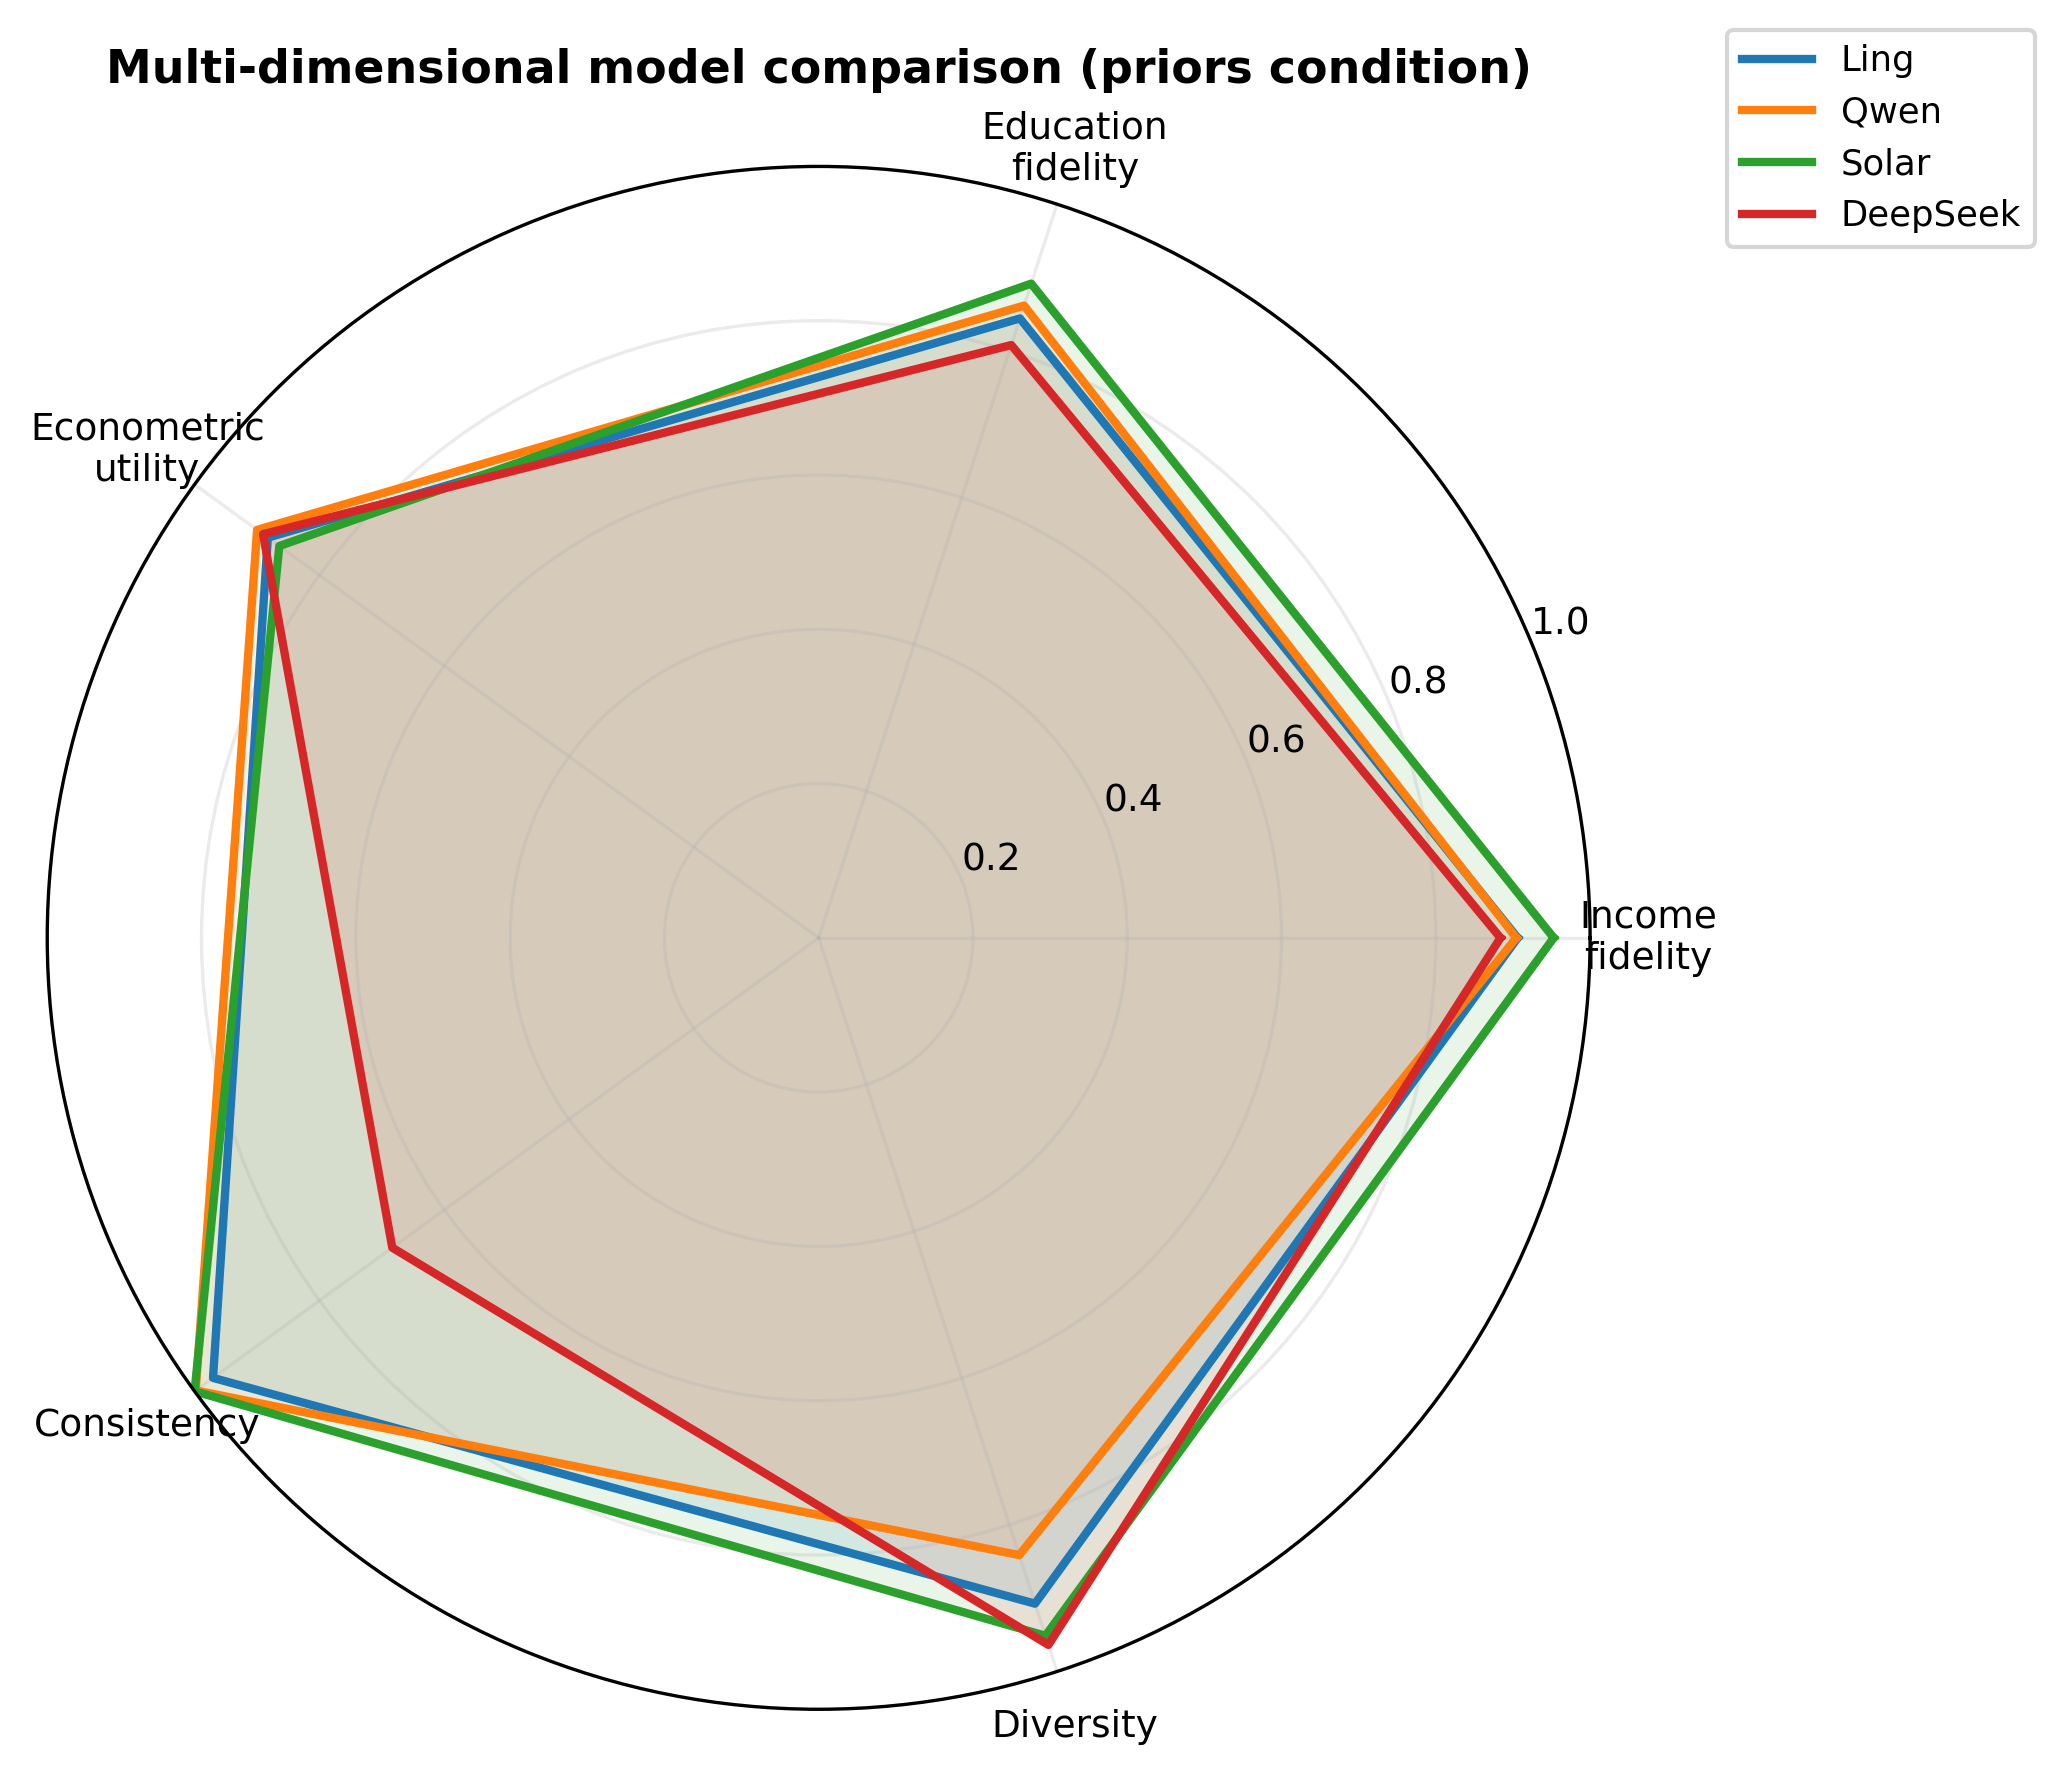
\includegraphics[width=0.72\linewidth]{figures/radar_comparison.png}
\caption{Multi-dimensional comparison of the four models (priors condition). Each axis is normalized to $[0,1]$; higher is better.}
\label{fig:radar}
\end{figure}

\begin{table}[htbp]
\centering
\caption{Cross-model fidelity comparison (priors condition) vs.\ baselines.}
\label{tab:cross_model}
\small
\begin{tabular}{lccccc}
\toprule
\textbf{Generator} & \textbf{MARE} & \textbf{TVD} & \textbf{W1$_\text{norm}$} & \textbf{Emp.\ rate} & \textbf{Unique} \\
\midrule
Ling 3.0 Flash     & 9.4\%  & 0.156 & 0.193 & 78.9\% & 90.8\% \\
DeepSeek V4 Flash  & 11.6\% & 0.192 & 0.149 & 61.6\% & 96.4\% \\
Qwen 3.7 Flash     & 9.6\%  & 0.138 & 0.157 & 82.6\% & 84.1\% \\
Solar Pro 4        & \textbf{4.7\%}  & \textbf{0.108} & 0.209 & 74.1\% & 95.1\% \\
\midrule
Uniform baseline   & 97.9\% & 0.260 & ---   & 50.4\% & 99.9\% \\
Marginal baseline  & 2.9\%  & 0.019 & ---   & 97.2\% & 100\%  \\
\midrule
\textbf{Reference} & ---    & ---   & ---   & 63.0\% & ---    \\
\bottomrule
\end{tabular}
\end{table}

\subsection{Income Fidelity}

\begin{figure}[htbp]
\centering
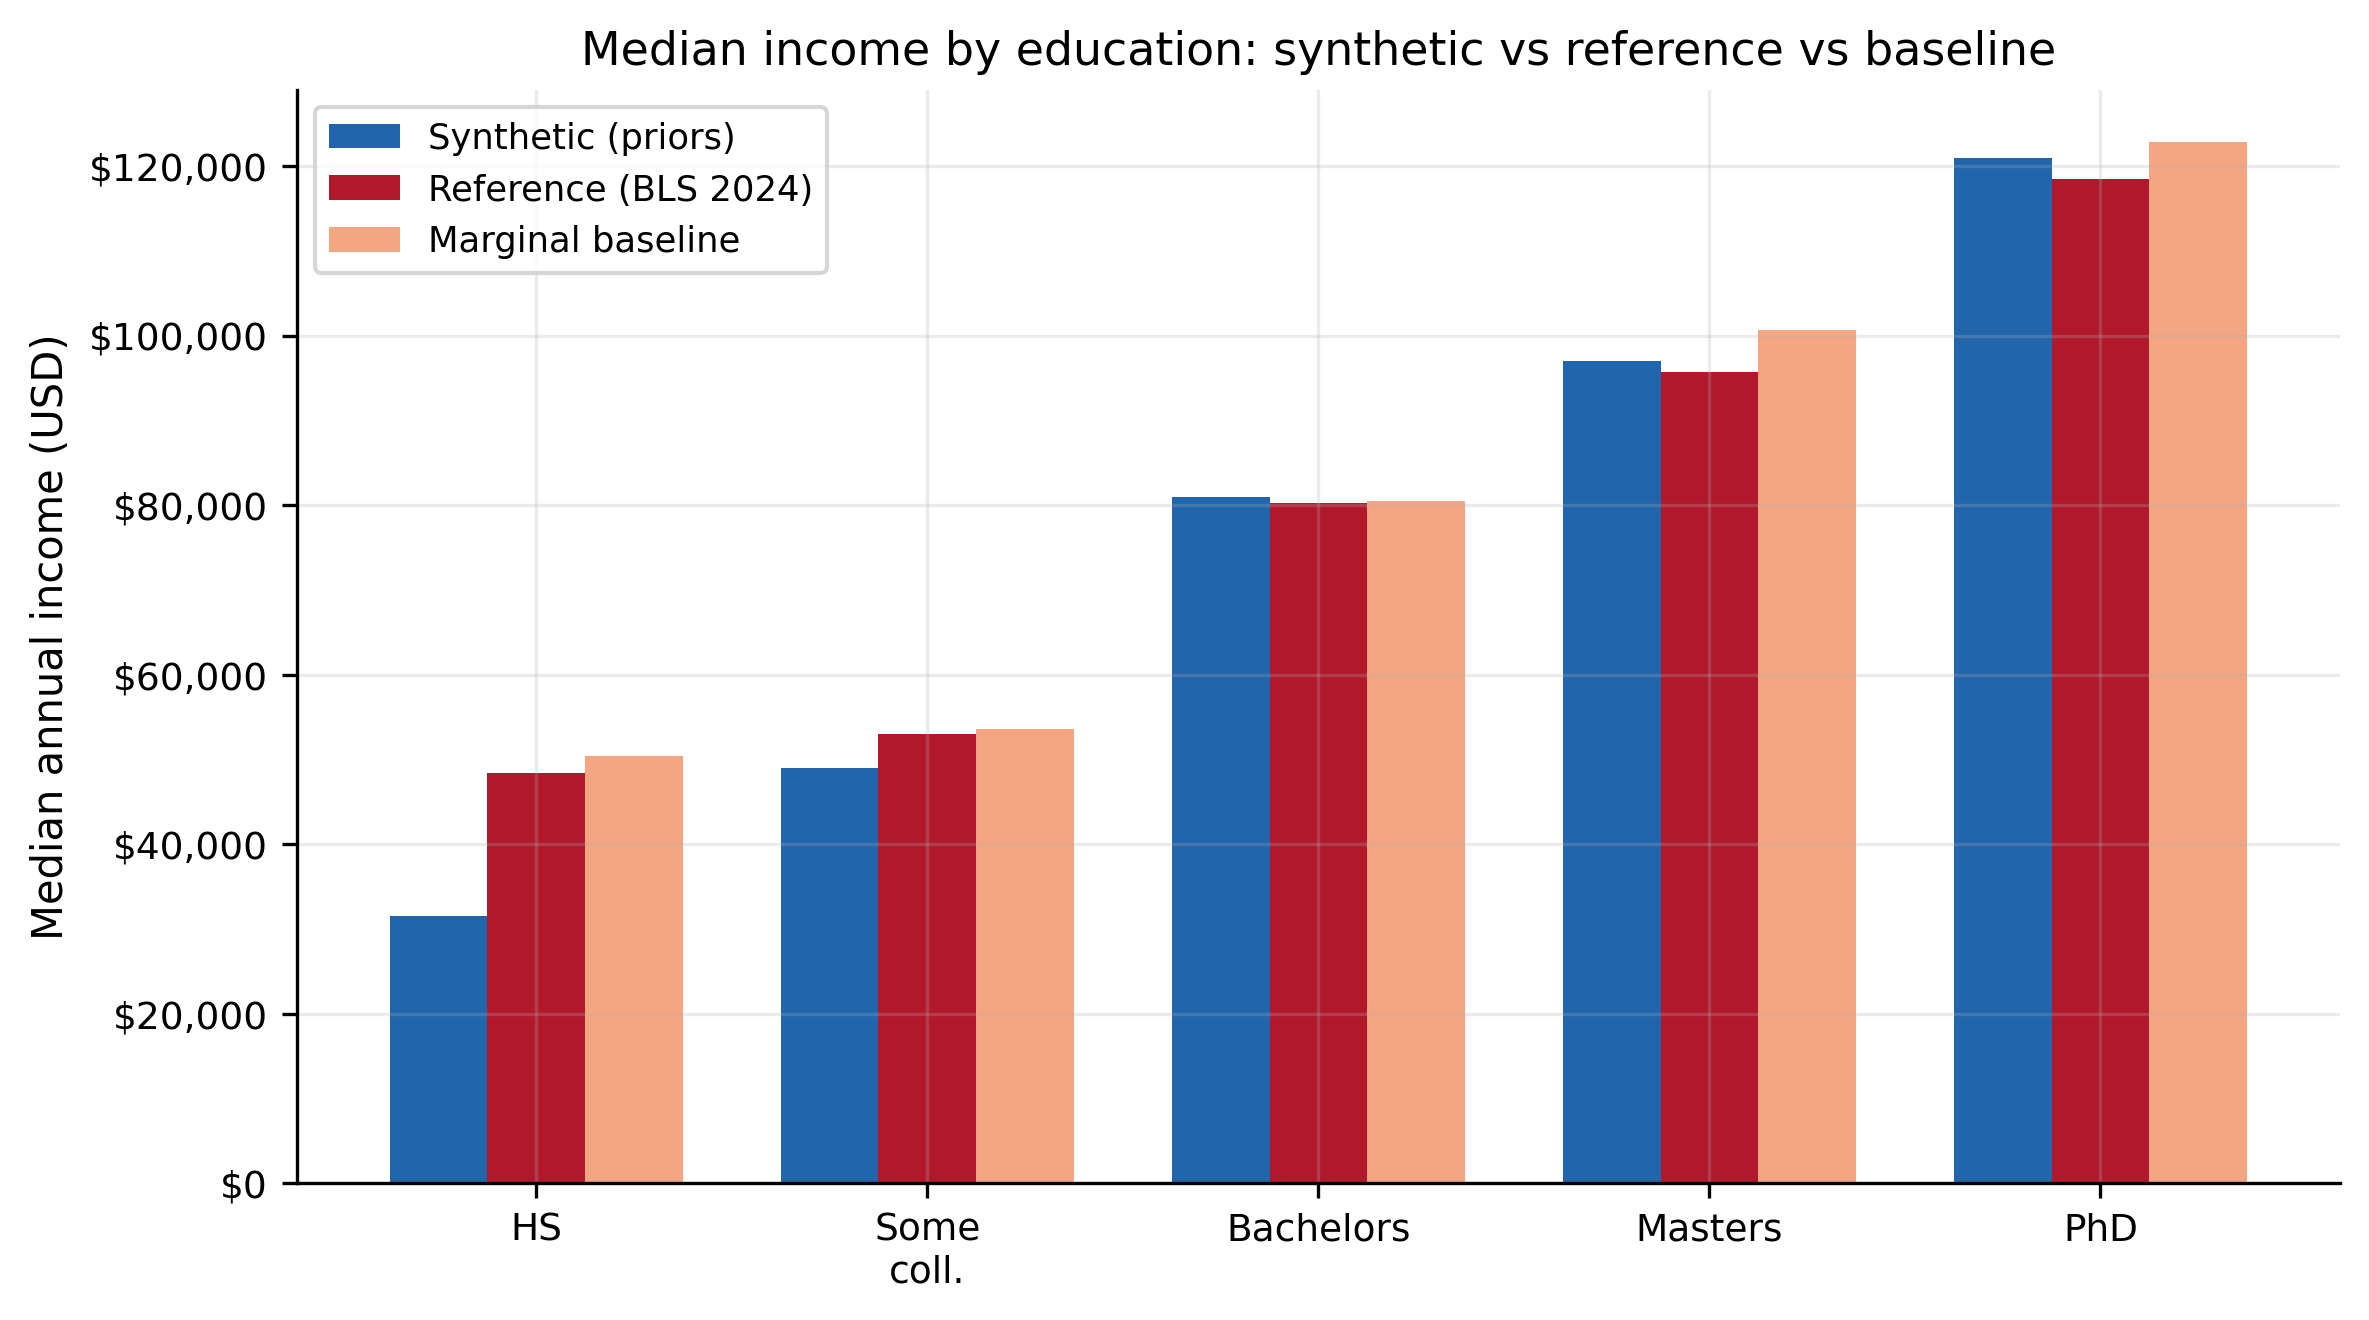
\includegraphics[width=0.85\linewidth]{figures/median_income.png}
\caption{Median annual income by education: Solar Pro 4 (priors) vs.\ BLS 2024 reference and the marginal baseline.}
\label{fig:income}
\end{figure}

Table~\ref{tab:income} compares synthetic and reference median income by education for the best-performing model (Solar Pro 4, priors condition).
The model reproduces the education--income gradient with a mean absolute relative error of 4.7\% (95\% CI [3.5\%, 5.3\%]).
Errors are smallest for bachelor's (1.0\%) and PhD (1.3\%) and largest for high school (13.2\%).

\begin{table}[htbp]
\centering
\caption{Median annual income by education: Solar Pro 4 (priors) vs.\ BLS reference.}
\label{tab:income}
\small
\begin{tabular}{lccc}
\toprule
\textbf{Education} & \textbf{Synthetic} & \textbf{Reference} & \textbf{Rel.\ err.} \\
\midrule
High school   & \$42{,}000 & \$48{,}360 & 13.2\% \\
Some college  & \$50{,}000 & \$53{,}040 & 5.7\%  \\
Bachelor's    & \$79{,}450 & \$80{,}236 & 1.0\%  \\
Master's      & \$98{,}000 & \$95{,}680 & 2.4\%  \\
PhD           & \$120{,}000 & \$118{,}456 & 1.3\% \\
\midrule
\multicolumn{3}{l}{Mean abs.\ relative error} & \textbf{4.7\%} \\
\multicolumn{3}{l}{95\% bootstrap CI} & {[}3.5\%, 5.3\%{]} \\
\bottomrule
\end{tabular}
\end{table}

\subsection{Downstream Econometric Utility}
\label{sec:results:utility}

\begin{figure}[htbp]
\centering
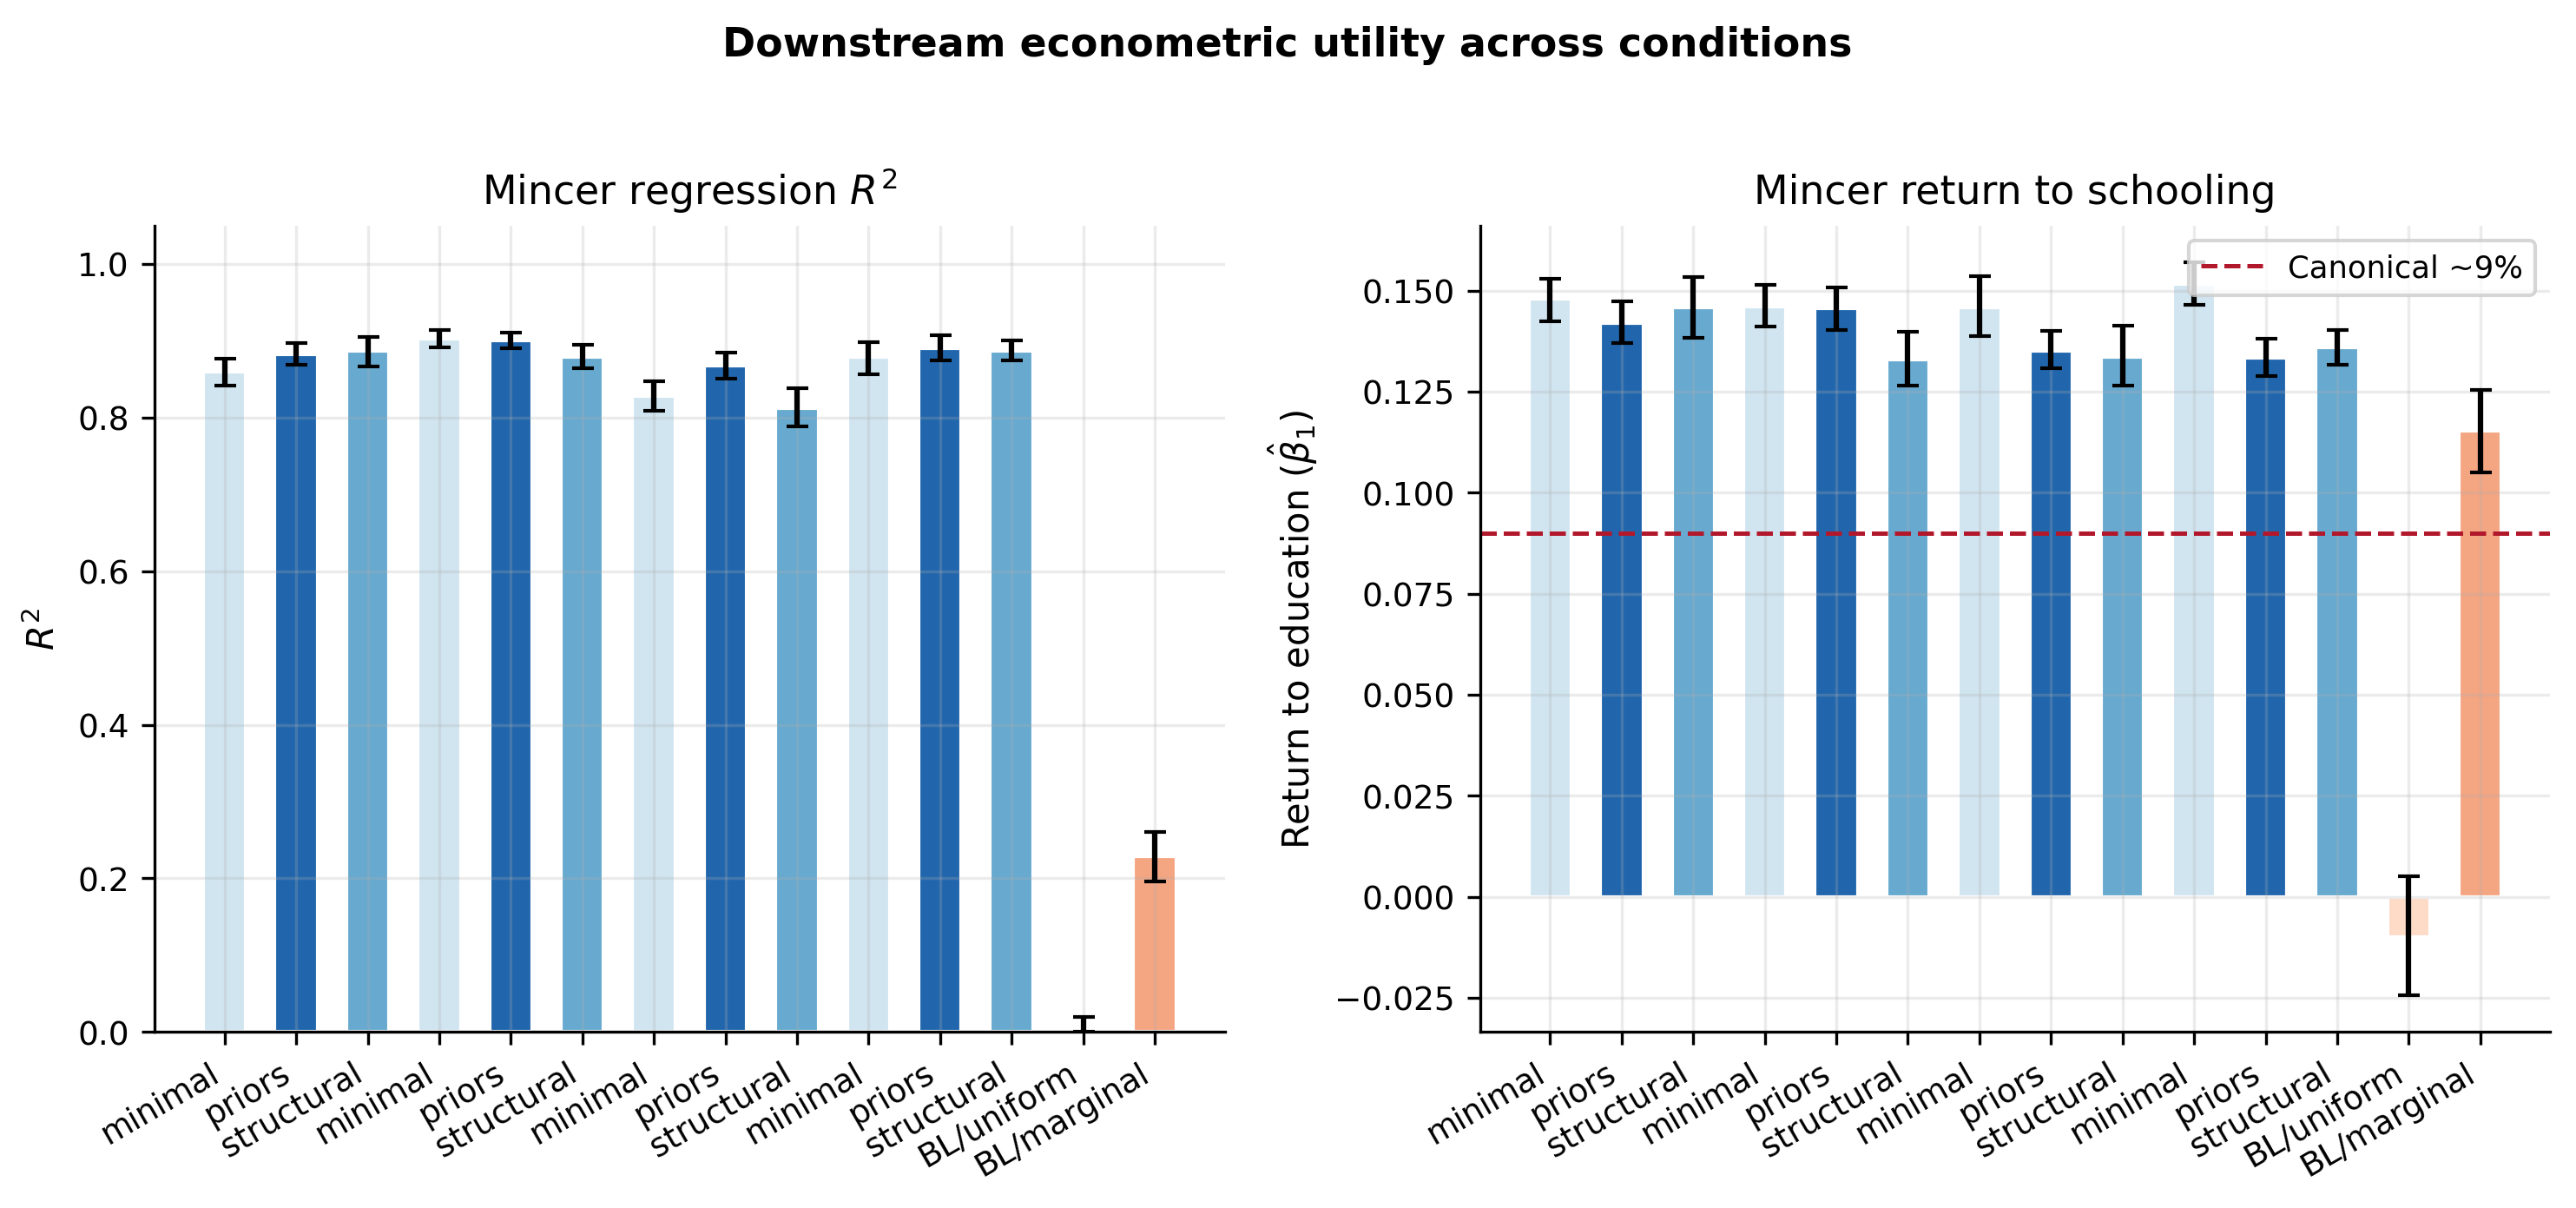
\includegraphics[width=0.9\linewidth]{figures/mincer_comparison.png}
\caption{Mincer regression $R^2$ and return to schooling across prompt conditions and baselines.}
\label{fig:mincer}
\end{figure}

Table~\ref{tab:mincer} reports the Mincer regression results for the priors condition across all four models.
All models recover a strong, statistically precise education--income relationship ($R^2 = 0.86$--0.90), with concave experience profiles (positive linear, negative quadratic term) consistent with the canonical age--earnings lifecycle.
However, the estimated returns to education (13.0--14.6\% per year) are systematically above the canonical 8--10\% range, reflecting the models' tendency to compress income differences into the education dimension.

\begin{table}[htbp]
\centering
\caption{Mincer wage regression on synthetic data (priors condition, employed workers).}
\label{tab:mincer}
\small
\begin{tabular}{lcccc}
\toprule
\textbf{Model} & \textbf{$n$} & \textbf{$R^2$} & \textbf{$\hat{\beta}_1$} & \textbf{95\% CI} \\
\midrule
Ling 3.0 Flash    & 631 & 0.883 & 0.142 & {[}0.137, 0.147{]} \\
DeepSeek V4 Flash & 493 & 0.890 & 0.133 & {[}0.129, 0.138{]} \\
Qwen 3.7 Flash    & 661 & 0.900 & 0.146 & {[}0.140, 0.151{]} \\
Solar Pro 4       & 593 & 0.864 & 0.134 & {[}0.130, 0.139{]} \\
\midrule
Canonical         & --- & ---   & 0.08--0.10 & --- \\
\bottomrule
\end{tabular}
\end{table}

\subsubsection{The Utility Advantage over Baselines}
\label{sec:baselines}

The decisive result is the comparison in Table~\ref{tab:utility}.
The marginal baseline, despite matching the marginals perfectly, fits a Mincer regression with only $R^2=0.23$ and a return-to-education of 11.7\%---because it has no joint structure linking education to income within the regression.
All four LLMs, by contrast, achieve $R^2 \geq 0.86$ with precisely estimated returns.
The uniform baseline is essentially uninformative ($R^2=0.004$).
This is the paper's central empirical claim: \emph{the LLMs' value is their conditional/joint structure, not their marginals}.

\begin{table}[htbp]
\centering
\caption{Downstream econometric utility: LLMs vs.\ baselines.}
\label{tab:utility}
\small
\begin{tabular}{lccc}
\toprule
\textbf{Generator} & \textbf{$R^2$} & \textbf{$\hat{\beta}_1$} & \textbf{$\hat{\beta}_1$ CI} \\
\midrule
Ling 3.0 Flash    & 0.883 & 0.142 & {[}0.137, 0.147{]} \\
DeepSeek V4 Flash & 0.890 & 0.133 & {[}0.129, 0.138{]} \\
Qwen 3.7 Flash    & 0.900 & 0.146 & {[}0.140, 0.151{]} \\
Solar Pro 4       & 0.864 & 0.134 & {[}0.130, 0.139{]} \\
\midrule
Uniform baseline  & 0.004 & $-0.010$ & --- \\
Marginal baseline & 0.229 & 0.117 & --- \\
\midrule
Canonical         & ---   & 0.08--0.10 & --- \\
\bottomrule
\end{tabular}
\end{table}

\subsubsection{Does the Proposed Remedy Work? A Calibration Demonstration}
\label{sec:calibration}

The comparison in Table~\ref{tab:utility} motivates a complementary division of labor: an LLM supplies the \emph{conditional} structure, while a lightweight post-processing step supplies the \emph{unconditional} marginals.
To make this recommendation concrete rather than aspirational, we implement the calibration step and measure its effect.
Specifically, we apply post-stratification weights to each synthetic dataset (priors condition) so that the weighted education distribution exactly matches the public Census shares---the marginal the models distort most (over-representing advanced degrees).
This requires only publicly available aggregate shares and no real records.
Figure~\ref{fig:calibration} and Table~\ref{tab:calibration} report the education-distribution TVD and the Mincer $R^2$ before and after calibration.

\begin{figure}[htbp]
\centering
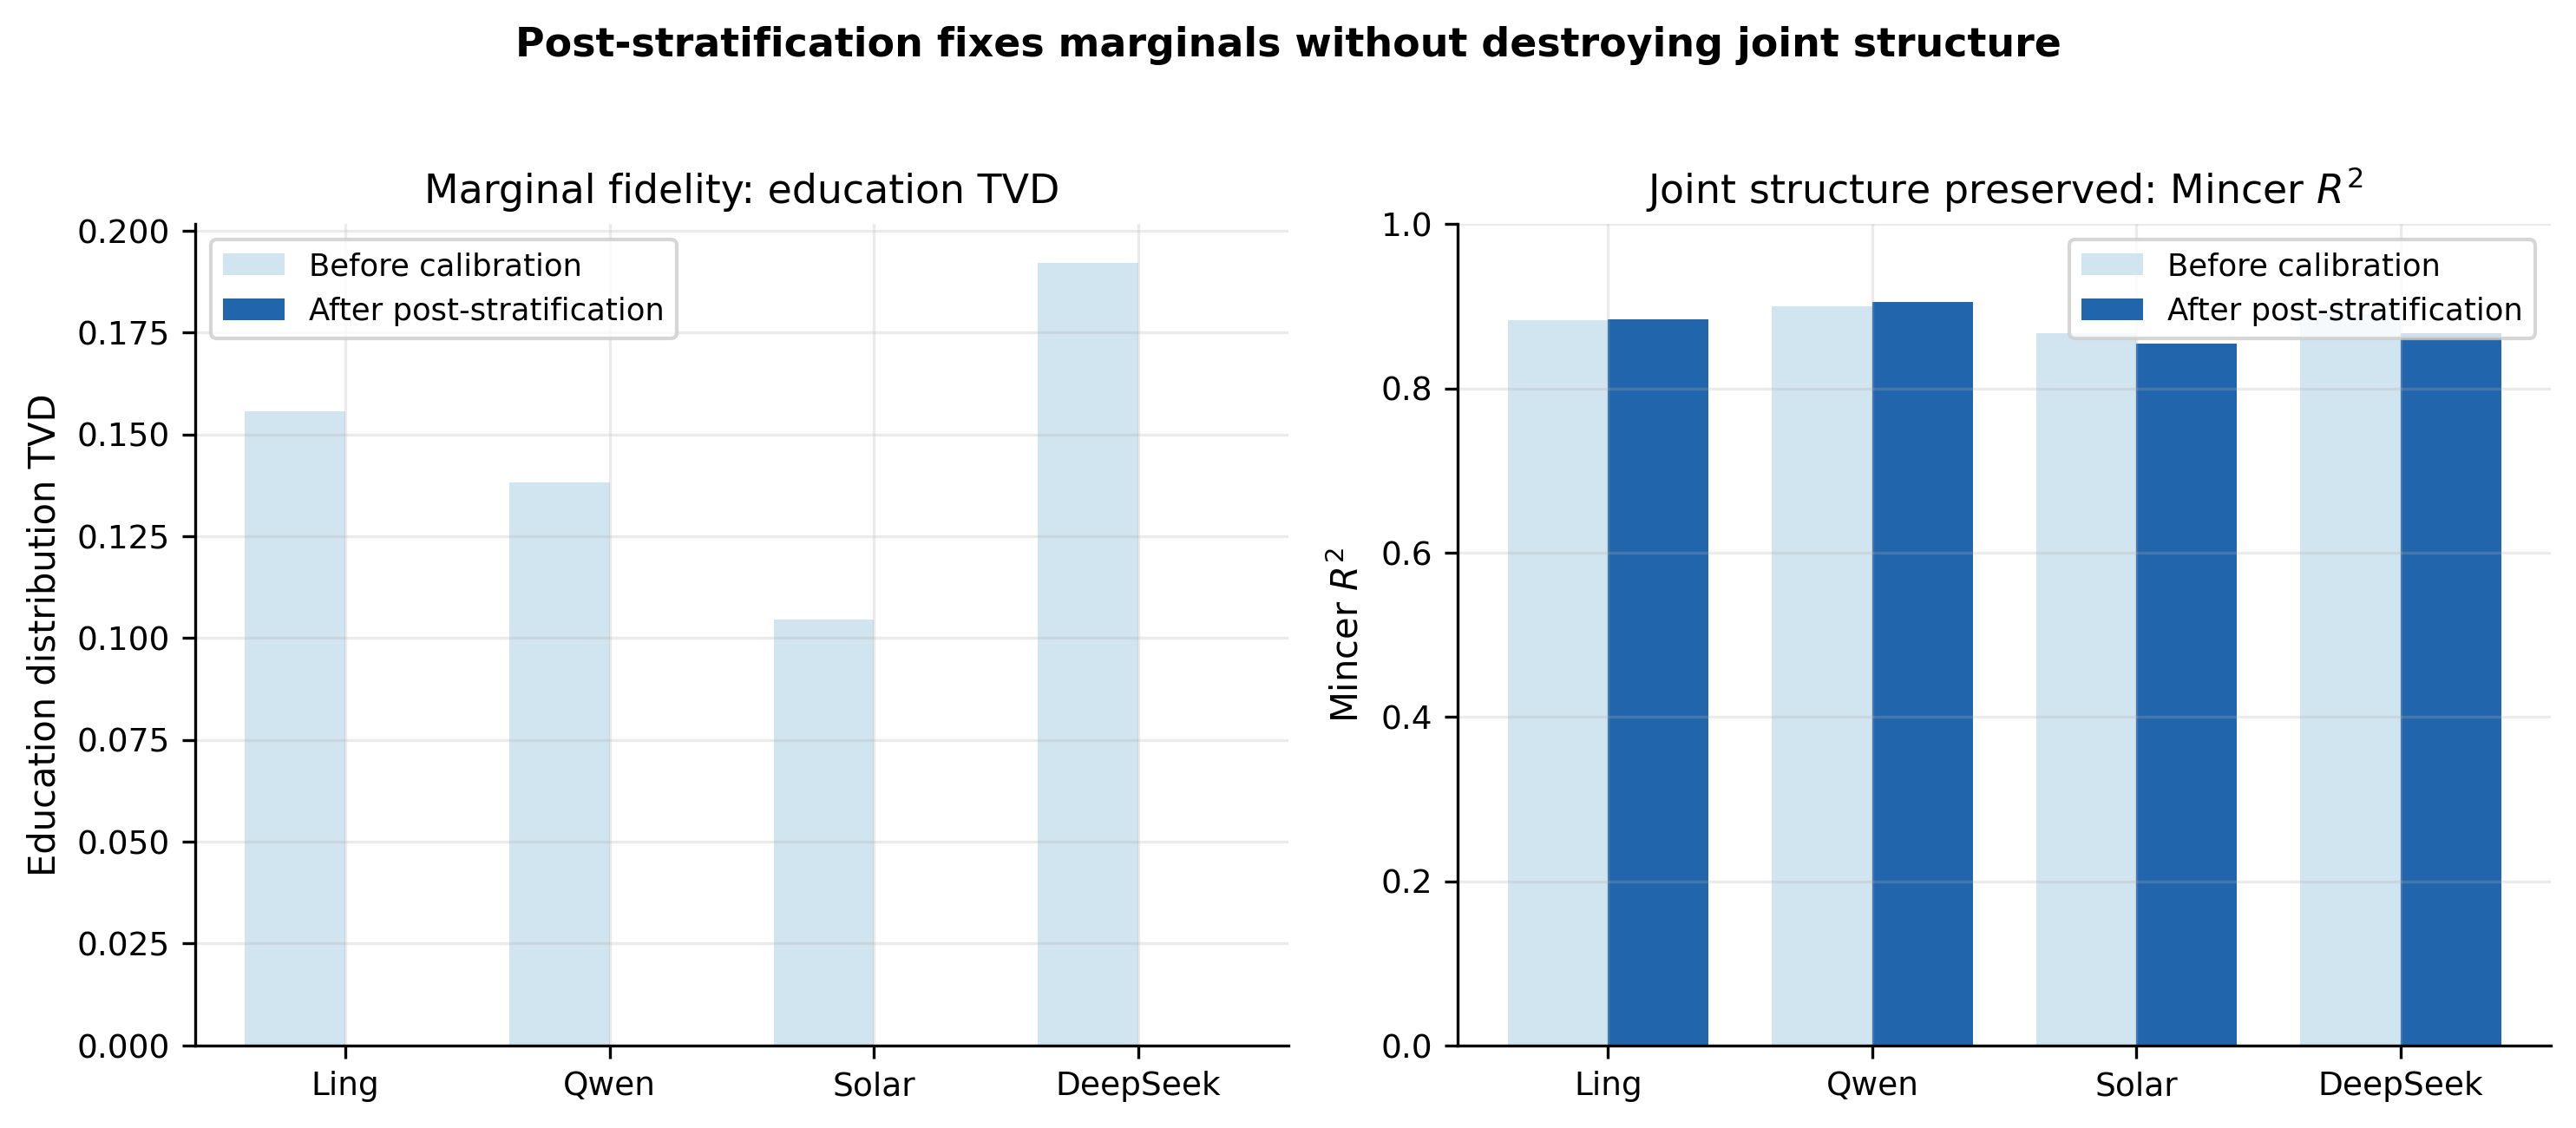
\includegraphics[width=0.95\linewidth]{figures/calibration_demo.png}
\caption{Post-stratification on the public education distribution reduces the education-distribution TVD to zero by construction while preserving the Mincer $R^2$ (changes within $\pm 0.02$). This validates the paper's central recommendation: LLM joint structure plus marginal calibration.}
\label{fig:calibration}
\end{figure}

\begin{table}[htbp]
\centering
\caption{Calibration demonstration: education TVD and Mincer $R^2$ before vs.\ after post-stratification (priors condition).}
\label{tab:calibration}
\small
\begin{tabular}{lcccc}
\toprule
\textbf{Model} & \textbf{TVD before} & \textbf{TVD after} & \textbf{$R^2$ before} & \textbf{$R^2$ after} \\
\midrule
Ling 3.0 Flash    & 0.156 & 0.000 & 0.883 & 0.884 \\
DeepSeek V4 Flash & 0.192 & 0.000 & 0.890 & 0.868 \\
Qwen 3.7 Flash    & 0.138 & 0.000 & 0.900 & 0.906 \\
Solar Pro 4       & 0.105 & 0.000 & 0.867 & 0.854 \\
\midrule
\textbf{Mean change} & --- & --- & --- & $\pm 0.02$ \\
\bottomrule
\end{tabular}
\end{table}

The result is decisive: post-stratification drives the education-distribution TVD to zero by construction, yet the Mincer $R^2$ changes by at most 0.02 (and in two of four models \emph{increases}), confirming that the joint structure is preserved under marginal reweighting.
This is the paper's central practical claim made testable: the LLM's contribution (conditional structure) and the calibration step's contribution (unconditional marginals) are complementary and do not interfere.
We note that employment remains a separate marginal to correct (the weighted employment rate is still elevated relative to the 63\% reference, since we calibrated only education); in practice a practitioner would rake on both marginals simultaneously, which is a straightforward extension of the same procedure.

\subsection{Prompt Ablation}
\label{sec:results:ablation}

Table~\ref{tab:ablation} presents the full ablation across all four models and three conditions.
The ablation reveals three key patterns:

\begin{enumerate}[leftmargin=*, itemsep=2pt]
  \item \textbf{Priors improve income fidelity.} Across all models, moving from \emph{minimal} to \emph{priors} reduces MARE by 40--53\% (e.g., Solar Pro 4: 21.7\% $\to$ 4.7\%; Ling 3.0 Flash: 16.7\% $\to$ 9.4\%).
  \item \textbf{Priors have limited effect on $R^2$.} The Mincer $R^2$ changes by less than 0.04 across conditions for each model, indicating that the joint structure is largely \emph{latent}---the models already encode the education--income correlation without explicit instruction.
  \item \textbf{Structural constraints improve consistency but not fidelity.} The \emph{structural} condition consistently improves the consistency metric $P(\text{income}=0 \mid \text{not employed})$ (e.g., Solar Pro 4: 37.3\% $\to$ 100.0\%) but does not reduce MARE and sometimes increases it.
\end{enumerate}

\begin{table}[htbp]
\centering
\caption{Prompt ablation: fidelity and utility across conditions and models.}
\label{tab:ablation}
\small
\begin{tabular}{llcccc}
\toprule
\textbf{Model} & \textbf{Condition} & \textbf{MARE} & \textbf{TVD} & \textbf{$R^2$} & \textbf{$\hat{\beta}_1$} \\
\midrule
\multirow{3}{*}{\shortstack[l]{Ling 3.0\\Flash}}
  & minimal    & 16.7\% & 0.176 & 0.860 & 0.148 \\
  & structural & 20.1\% & 0.209 & 0.886 & 0.146 \\
  & priors     & 9.4\%  & 0.156 & 0.883 & 0.142 \\
\midrule
\multirow{3}{*}{\shortstack[l]{DeepSeek\\V4 Flash}}
  & minimal    & 18.1\% & 0.184 & 0.878 & 0.152 \\
  & structural & 24.9\% & 0.222 & 0.887 & 0.136 \\
  & priors     & 11.6\% & 0.192 & 0.890 & 0.133 \\
\midrule
\multirow{3}{*}{\shortstack[l]{Qwen 3.7\\Flash}}
  & minimal    & 18.7\% & 0.186 & 0.902 & 0.146 \\
  & structural & 19.6\% & 0.201 & 0.879 & 0.133 \\
  & priors     & 9.6\%  & 0.138 & 0.900 & 0.146 \\
\midrule
\multirow{3}{*}{\shortstack[l]{Solar\\Pro 4}}
  & minimal    & 21.7\% & 0.121 & 0.828 & 0.146 \\
  & structural & 19.8\% & 0.165 & 0.812 & 0.134 \\
  & priors     & \textbf{4.7\%}  & \textbf{0.108} & 0.864 & 0.134 \\
\midrule
\multicolumn{2}{l}{Uniform baseline}  & 97.9\% & 0.260 & 0.004 & $-0.010$ \\
\multicolumn{2}{l}{Marginal baseline} & 2.9\%  & 0.019 & 0.229 & 0.117 \\
\bottomrule
\end{tabular}
\end{table}

\subsection{Internal Consistency}

Table~\ref{tab:consistency} reports internal consistency metrics for the priors condition.
All models achieve near-perfect consistency on the employment--hours dimension: every employed record has positive hours and every non-employed record has zero hours.
The weakest consistency dimension is $P(\text{income}=0 \mid \text{not employed})$, where Solar Pro 4 achieves 100\% and DeepSeek V4 Flash only 36.2\%, indicating that DeepSeek frequently assigns nonzero income to non-employed records.

\begin{table}[htbp]
\centering
\caption{Internal consistency of synthetic records (priors condition).}
\label{tab:consistency}
\small
\begin{tabular}{lcccc}
\toprule
\textbf{Condition} & \textbf{Ling} & \textbf{DeepSeek} & \textbf{Qwen} & \textbf{Solar} \\
\midrule
$\text{hours}>0 \mid \text{employed}$ & 100\% & 100\% & 100\% & 100\% \\
$\text{hours}=0 \mid \text{not emp.}$ & 100\% & 100\% & 100\% & 100\% \\
$\text{income}>0 \mid \text{employed}$ & 100\% & 100\% & 100\% & 100\% \\
$\text{income}=0 \mid \text{not emp.}$ & 88.2\% & 36.2\% & 99.3\% & 100\% \\
Monotone in education & Yes & Yes & Yes & Yes \\
\bottomrule
\end{tabular}
\end{table}

\subsection{Diversity}

All models exhibit substantial diversity: unique record ratios range from 84.1\% (Qwen) to 96.4\% (DeepSeek), and Shannon entropy across categorical fields indicates no degenerate repetition (gender entropy $\approx 0.69$, the theoretical maximum for a balanced binary split).

\subsection{The Unemployment Failure Mode}

The most severe and consistent distortion is in the unemployment-by-education marginals.
\begin{figure}[htbp]
\centering
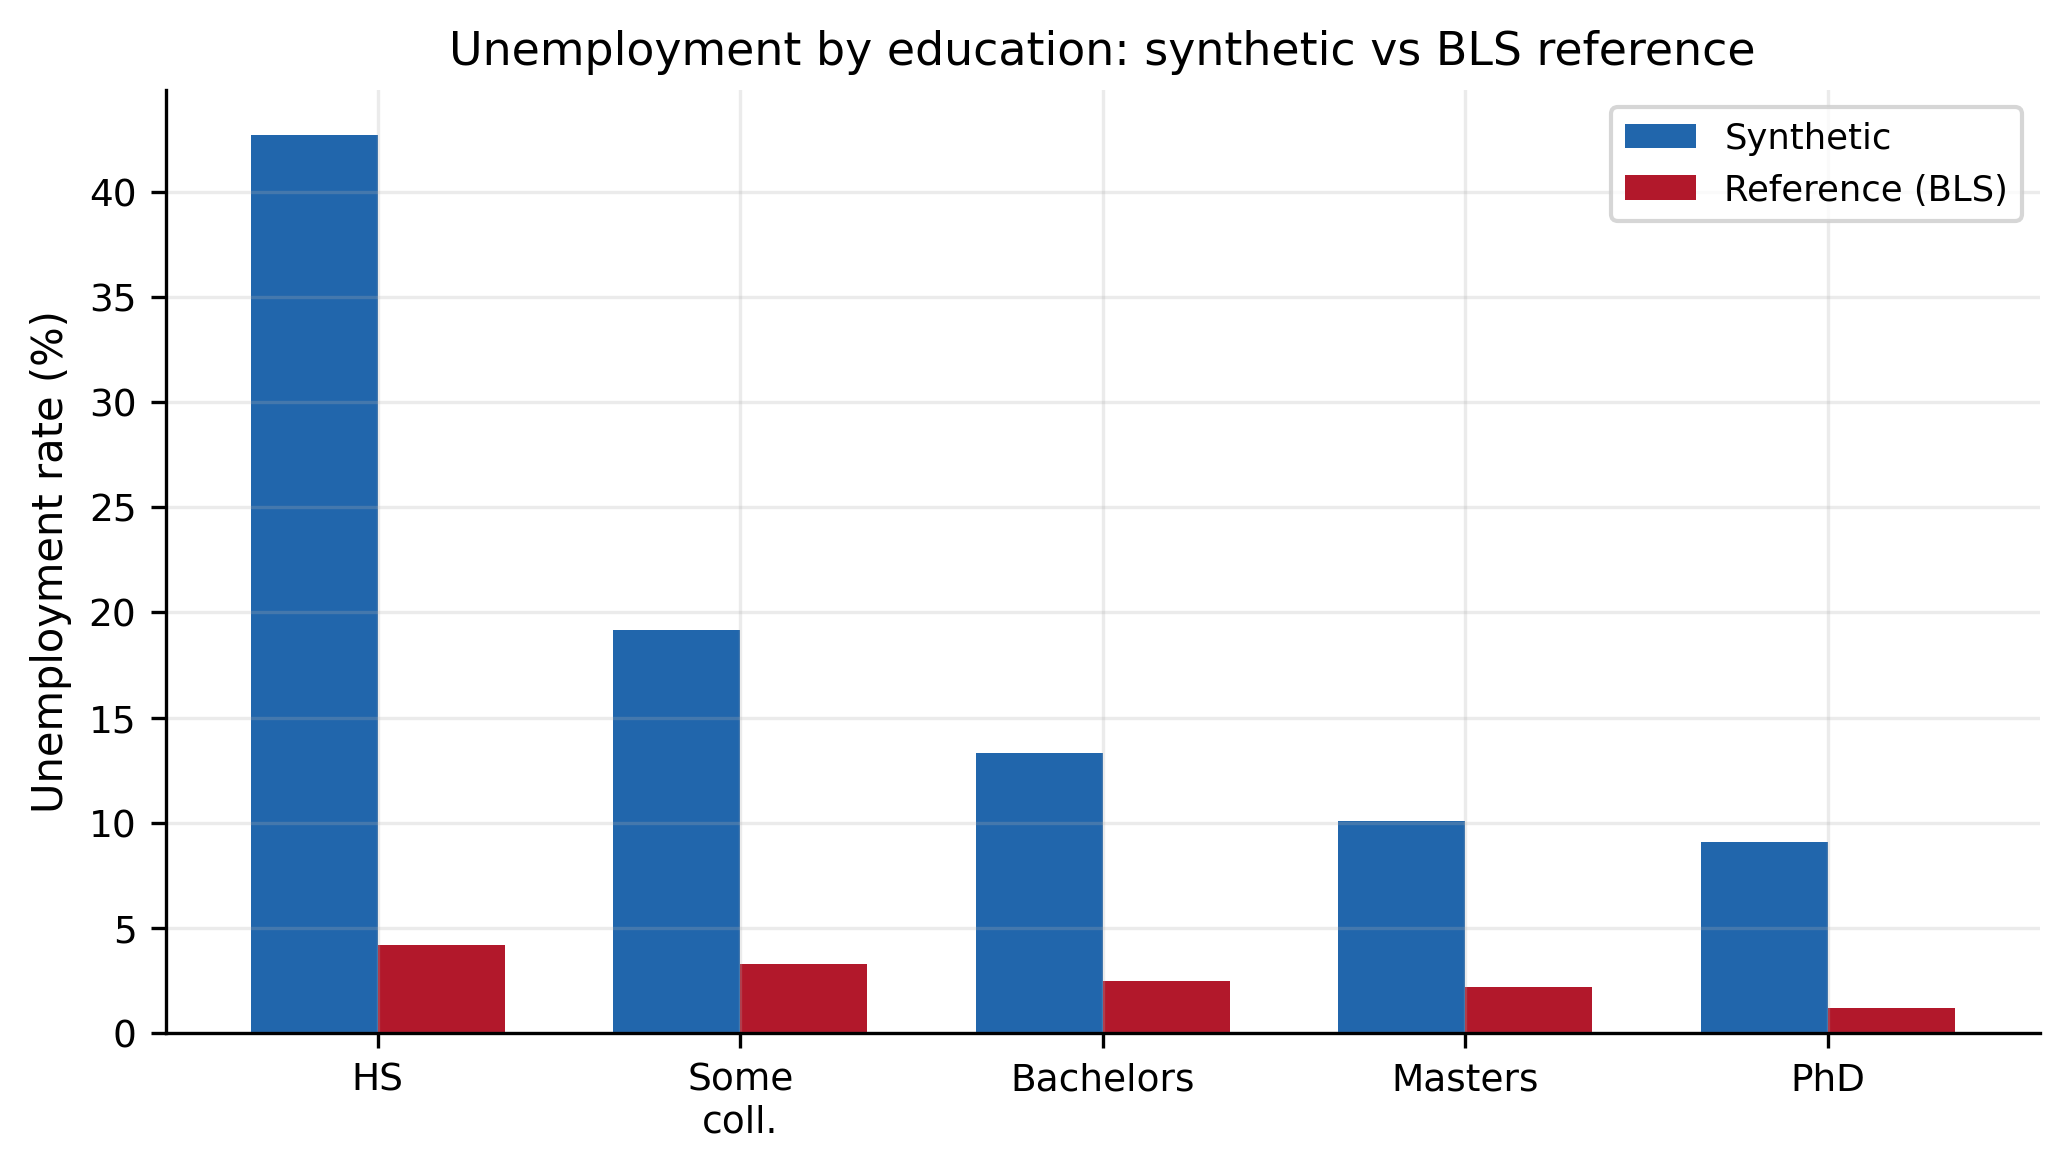
\includegraphics[width=0.85\linewidth]{figures/unemployment_by_education.png}
\caption{Unemployment by education: synthetic (priors) vs.\ BLS reference. The models dramatically overstate unemployment for lower education levels.}
\label{fig:unemp}
\end{figure}
Table~\ref{tab:unemployment} shows that all models dramatically overstate unemployment for lower education levels, with MAREs ranging from 3.6$\times$ to 8.3$\times$ the reference values.
Notably, the \emph{priors} condition does not reliably improve---and sometimes worsens---this distortion, suggesting that the models lack accurate latent knowledge of population-level unemployment rates.

\begin{table}[htbp]
\centering
\caption{Unemployment by education: synthetic (priors) vs.\ BLS reference (\%).}
\label{tab:unemployment}
\small
\begin{tabular}{lccccc}
\toprule
\textbf{Education} & \textbf{Ref.} & \textbf{Ling} & \textbf{DeepSeek} & \textbf{Qwen} & \textbf{Solar} \\
\midrule
High school   & 4.2 & 42.7 & 46.9 & 32.4 & 48.0 \\
Some college  & 3.8 & 19.2 & 38.6 & 20.0 & 21.0 \\
Bachelor's    & 2.5 & 13.3 & 38.8 & 12.6 & 11.6 \\
Master's      & 2.2 & 10.1 & 34.6 & 5.0  & 13.3 \\
PhD           & 1.2 & 9.1  & 28.7 & 2.4  & 21.5 \\
\midrule
\textbf{MARE}     & --- & 5.7$\times$ & 14.6$\times$ & 3.6$\times$ & 8.3$\times$ \\
\bottomrule
\end{tabular}
\end{table}

\subsection{Cross-Model Agreement}

Table~\ref{tab:jsd} reports the pairwise Jensen--Shannon divergence between models.
The education distributions are remarkably similar across all model pairs (JSD $< 0.009$), indicating strong agreement on the population's educational composition.
Income distributions show more variation (JSD 0.02--0.05), reflecting model-specific differences in income calibration.

\begin{table}[htbp]
\centering
\caption{Pairwise Jensen--Shannon divergence (priors condition).}
\label{tab:jsd}
\small
\begin{tabular}{lcc}
\toprule
\textbf{Model pair} & \textbf{Education JSD} & \textbf{Income JSD} \\
\midrule
Ling vs.\ Qwen       & 0.0003 & 0.034 \\
Ling vs.\ Solar       & 0.0020 & 0.033 \\
Ling vs.\ DeepSeek    & 0.0028 & 0.040 \\
Qwen vs.\ Solar       & 0.0010 & 0.052 \\
Qwen vs.\ DeepSeek    & 0.0048 & 0.044 \\
Solar vs.\ DeepSeek   & 0.0082 & 0.020 \\
\midrule
\textbf{Mean}         & \textbf{0.0032} & \textbf{0.037} \\
\bottomrule
\end{tabular}
\end{table}

\subsection{Seed Stability and Reproducibility}

Table~\ref{tab:stability} reports the coefficient of variation (CV) of key metrics across two random seeds.
The Mincer $R^2$ is remarkably stable: CV $< 3.5\%$ for all (model, condition) pairs, with most below 2\%.
MARE shows more variation (CV up to 12.6\% for Solar Pro 4/priors), but this reflects the inherently higher variance of quantile-based metrics on small samples rather than instability in the generation process.
The return to education ($\hat{\beta}_1$) is also stable, with CV $< 4\%$ across all conditions.
Figure~\ref{fig:stability} visualizes this stability, confirming that the econometric utility of the synthetic data is not an artifact of a particular random seed.

\begin{figure}[htbp]
\centering
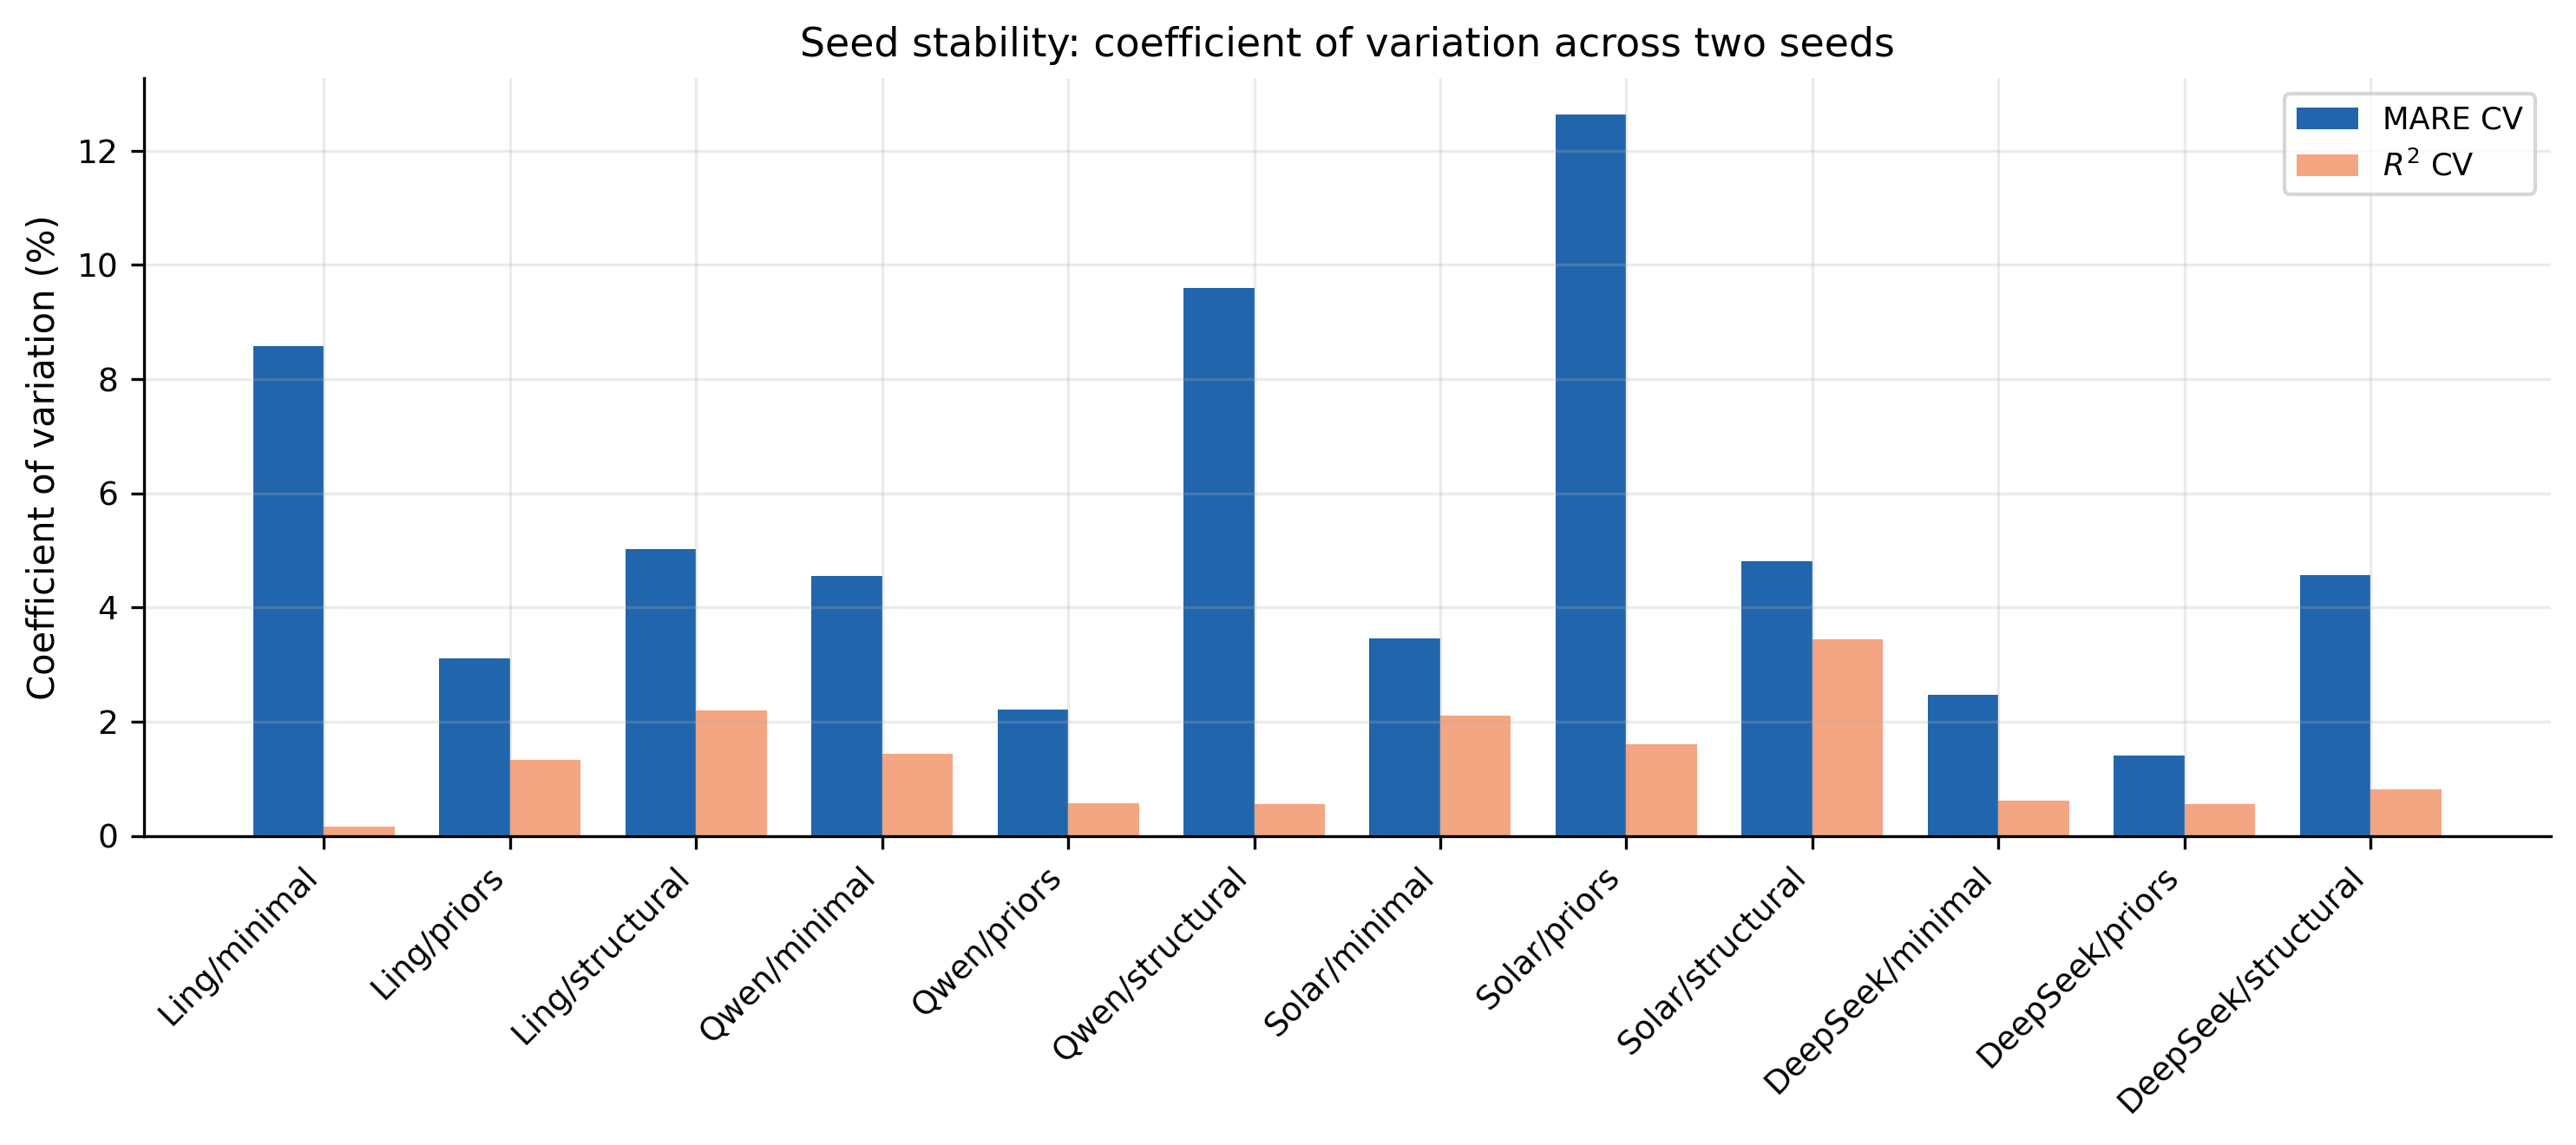
\includegraphics[width=0.9\linewidth]{figures/seed_stability.png}
\caption{Coefficient of variation of MARE and Mincer $R^2$ across two random seeds, by model and condition.}
\label{fig:stability}
\end{figure}

\begin{table}[htbp]
\centering
\caption{Seed stability: coefficient of variation (CV) across two seeds.}
\label{tab:stability}
\small
\begin{tabular}{llccccc}
\toprule
\textbf{Model} & \textbf{Cond.} & \textbf{MARE CV} & \textbf{$R^2$ CV} & \textbf{$\hat{\beta}_1$ CV} & \textbf{TVD CV} & \textbf{Emp.\ CV} \\
\midrule
\multirow{3}{*}{\shortstack[l]{Ling}}
  & min.  & 8.6\%  & 0.2\%  & 1.5\%  & 1.0\%  & 0.0\%  \\
  & str.  & 5.0\%  & 2.2\%  & 3.0\%  & 5.1\%  & 1.2\%  \\
  & priors & 3.1\% & 1.3\%  & 3.2\%  & 1.1\%  & 0.2\%  \\
\midrule
\multirow{3}{*}{\shortstack[l]{DeepSeek}}
  & min.  & 2.5\%  & 0.6\%  & 3.2\%  & 3.8\%  & 0.4\%  \\
  & str.  & 4.6\%  & 0.8\%  & 2.2\%  & 9.6\%  & 4.1\%  \\
  & priors & 1.4\% & 0.6\%  & 3.6\%  & 1.8\%  & 3.7\%  \\
\midrule
\multirow{3}{*}{\shortstack[l]{Qwen}}
  & min.  & 4.6\%  & 1.4\%  & 0.6\%  & 1.0\%  & 0.7\%  \\
  & str.  & 9.6\%  & 0.6\%  & 6.8\%  & 2.6\%  & 1.2\%  \\
  & priors & 2.2\% & 0.6\%  & 1.4\%  & 6.4\%  & 1.1\%  \\
\midrule
\multirow{3}{*}{\shortstack[l]{Solar}}
  & min.  & 3.5\%  & 2.1\%  & 2.5\%  & 4.4\%  & 2.0\%  \\
  & str.  & 4.8\%  & 3.4\%  & 1.4\%  & 2.2\%  & 0.3\%  \\
  & priors & 12.6\% & 1.6\% & 1.9\%  & 6.8\%  & 0.5\%  \\
\bottomrule
\end{tabular}
\end{table}

\subsection{Gender Pay Gap Analysis}

Table~\ref{tab:gender} reports the synthetic gender pay gap compared to the BLS reference of approximately 16\%.
None of the models reproduce the full magnitude of the gender pay gap; the largest synthetic gap is 8.8\% (DeepSeek V4 Flash), roughly half the reference.
Two models (Ling, Qwen) show effectively zero gap, and the marginal baseline shows only 3.0\%.
This is consistent with our broader finding that models encode \emph{conditional} structure (education$\rightarrow$income) but not \emph{unconditional} demographic patterns (gender$\rightarrow$income).
Figure~\ref{fig:gender} visualizes this gap.

\begin{figure}[htbp]
\centering
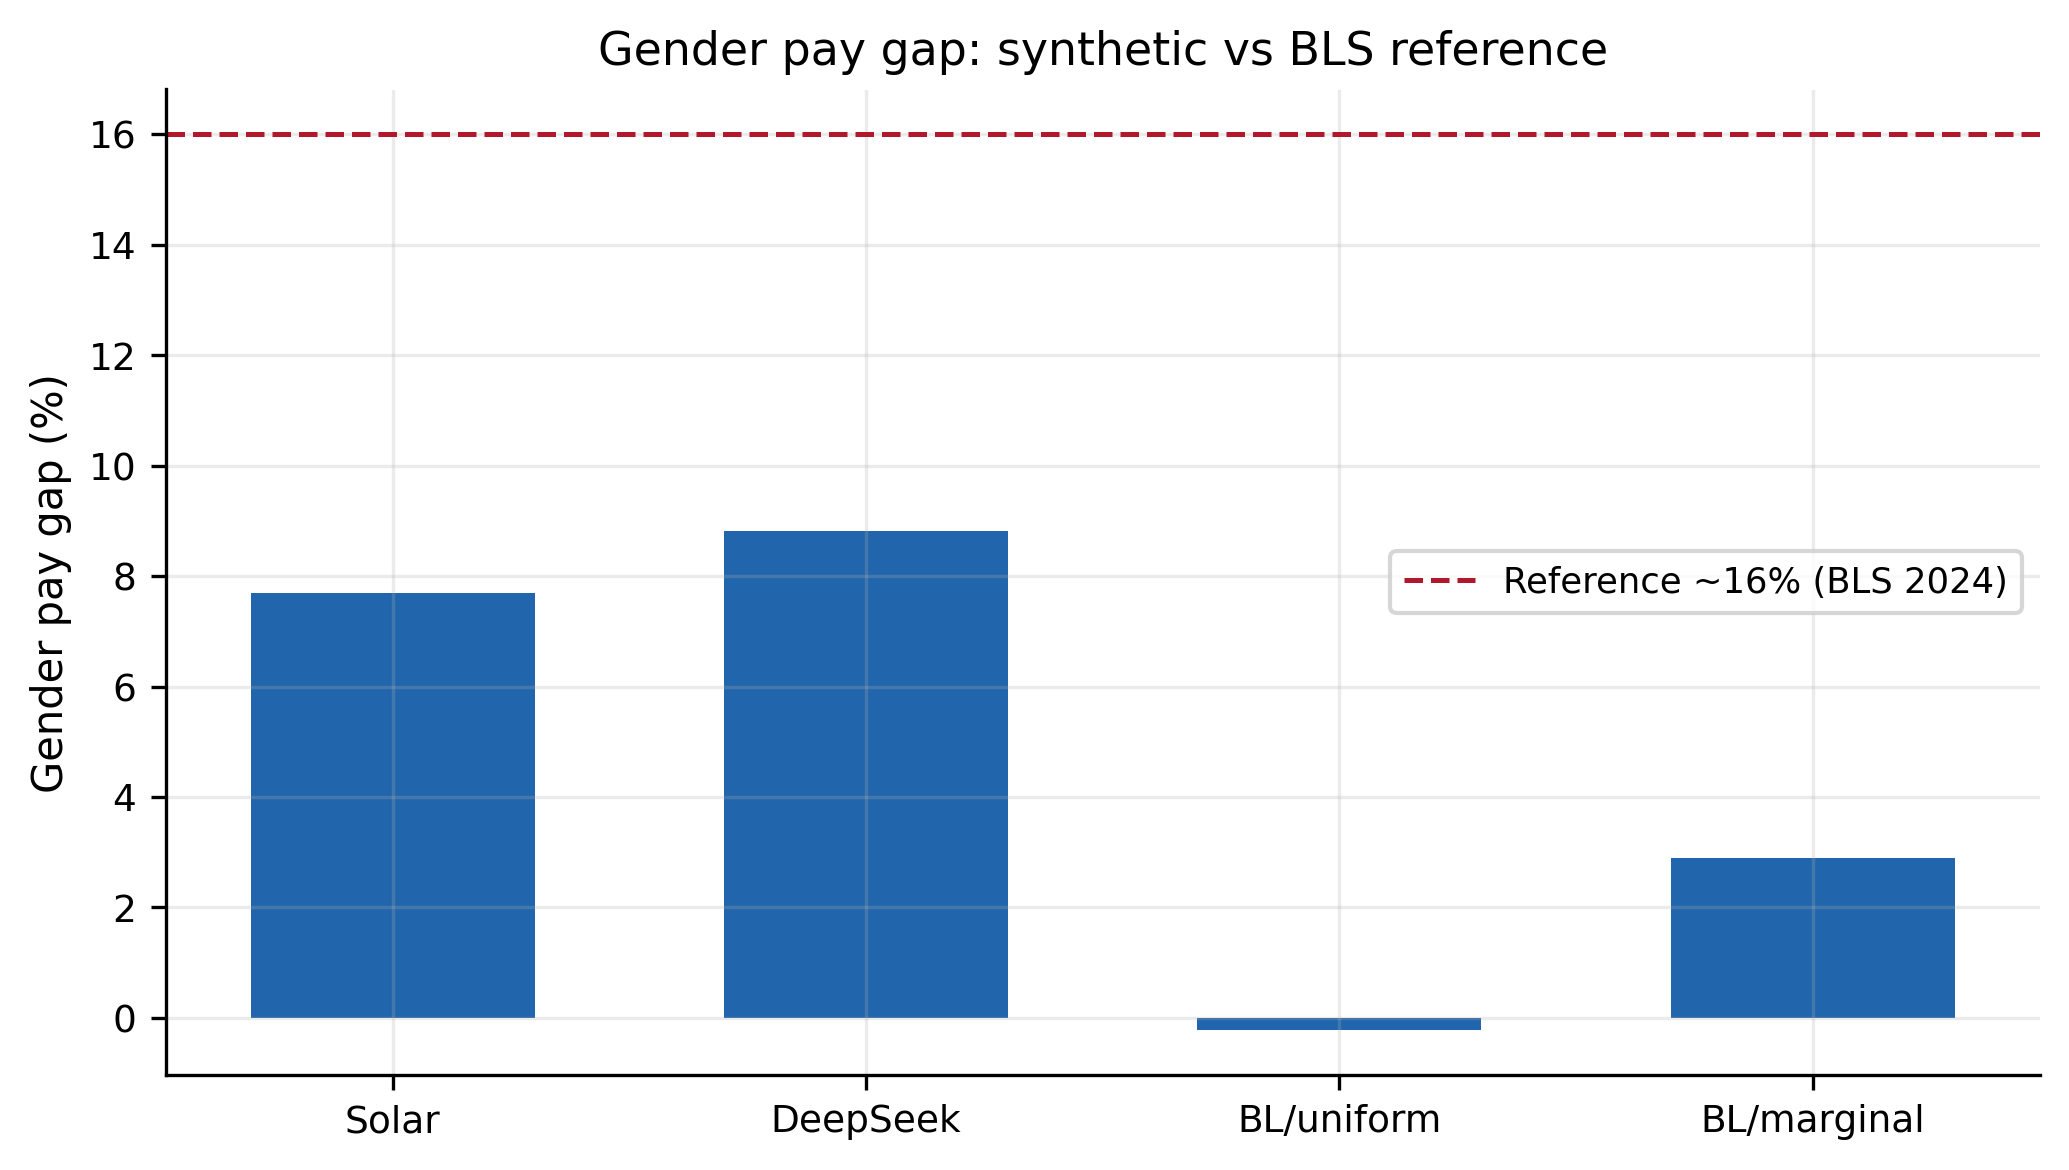
\includegraphics[width=0.72\linewidth]{figures/gender_gap.png}
\caption{Gender pay gap across models (priors condition) vs.\ the BLS 2024 reference of approximately 16\%.}
\label{fig:gender}
\end{figure}

\begin{table}[htbp]
\centering
\caption{Gender pay gap: synthetic vs.\ BLS 2024 reference.}
\label{tab:gender}
\small
\begin{tabular}{lccccc}
\toprule
\textbf{Generator} & \textbf{Male med.} & \textbf{Female med.} & \textbf{Gap} & \textbf{$n_M$} & \textbf{$n_F$} \\
\midrule
Ling 3.0 Flash    & \$78{,}000 & \$78{,}000 & $<1$\% & 318 & 313 \\
DeepSeek V4 Flash & \$68{,}000 & \$62{,}000 & 8.8\%  & 245 & 248 \\
Qwen 3.7 Flash    & \$65{,}000 & \$65{,}000 & $<1$\% & 326 & 335 \\
Solar Pro 4       & \$78{,}000 & \$72{,}000 & 7.7\%  & 310 & 288 \\
\midrule
Marginal baseline & \$62{,}640 & \$60{,}776 & 3.0\%  & 827 & 907 \\
\midrule
\textbf{Reference} & --- & --- & \textbf{$\sim$16\%} & --- & --- \\
\bottomrule
\end{tabular}
\end{table}

% ══════════════════════════════════════════════════════════════════════
% 5. DISCUSSION
% ══════════════════════════════════════════════════════════════════════
\section{Discussion}
\label{sec:discussion}

\subsection{Interpretation}

The central finding is a sharp asymmetry: small LLMs reproduce \emph{conditional} economic structure with high fidelity while distorting \emph{unconditional} marginals.
The education--income gradient, the employment--hours--income consistency, and the concave age--earnings profile are all captured well, as evidenced by MAREs of 4.7--11.6\% and Mincer $R^2$ values of 0.86--0.90.
Yet the models overstate the employment rate (62--83\% vs.\ 63\%), overstate advanced degrees (PhD 8.8--11.8\% vs.\ 3.3\%), and dramatically distort unemployment rates.

This pattern is consistent with the models' prior knowledge being \emph{relational} rather than \emph{population-level}: they know that more education implies more income and that employed people work, but they do not encode the base rates of employment or degree attainment in the adult population.
The cross-model JSD analysis (Table~\ref{tab:jsd}) reinforces this: all four models converge on very similar education distributions (JSD $< 0.009$) yet diverge on income (JSD 0.02--0.05), suggesting that the education--income mapping is the primary axis of latent knowledge, while the absolute income levels are harder to calibrate.
This is a useful, actionable characterization: conditional relationships are the model's strength, and unconditional marginals are its weakness.

\subsubsection{Why Conditional but Not Marginal Knowledge?}

This asymmetry admits a natural explanation grounded in how language models are trained.
Conditional relationships---``more education is associated with higher earnings,'' ``employed people work,'' ``income rises with age then falls''---are \emph{relational} statements that recur across the vast corpus of economic writing, journalism, and policy documents on which the models were trained.
They are robust to the exact base rates because they are stated as qualitative regularities, not as precise population shares.
Unconditional marginals, by contrast, are \emph{population-level} facts---the fraction of adults with a PhD, the employment-population ratio---that are (i)~time-varying, (ii)~country-specific, and (iii)~rarely stated as precise numbers in the training corpus.
A model asked to generate ``a realistic US population'' therefore defaults to a stylized, idealized population in which educational attainment and employment are higher than in the actual CPS, because the qualitative priors it has absorbed describe a more educated, more employed population than the real one.

This interpretation is consistent with the specific failure modes we observe.
The models over-represent advanced degrees (PhD 8.8--11.8\% vs.\ 3.3\%)---consistent with a training corpus that discusses PhD holders far more than their 3.3\% population share would warrant.
They overstate the employment rate (62--83\% vs.\ 63\%)---consistent with a corpus that describes people in terms of their jobs.
And they dramatically overstate unemployment for lower education levels---consistent with a conflation of the \emph{unemployment rate} (a conditional statistic among labor-force participants) with the \emph{non-employment rate} (a population-level statistic that includes retirees, students, and homemakers).
The models appear to encode the qualitative direction of these relationships without the quantitative base rates, which is precisely the boundary our ablation and calibration analyses identify.

\subsection{What the Baselines Reveal}

The comparison with non-LLM baselines sharpens the interpretation.
The \emph{marginal} baseline, which is handed the correct marginals, trivially beats the LLMs on MARE (2.9\% vs.\ 4.7--11.6\%) and TVD (0.02 vs.\ 0.11--0.19)---but it fails to capture any joint structure, fitting a Mincer regression with only $R^2=0.23$.
The LLMs, despite their distorted marginals, capture the joint structure that matters for econometric utility ($R^2 \geq 0.86$).
This suggests a complementary division of labor: a cheap LLM can supply the \emph{conditional} structure, while a lightweight post-processing step that reweights or resamples records to match known population marginals could supply the \emph{unconditional} marginals.
This hybrid---LLM-generated joint structure plus marginal calibration---is a promising and inexpensive direction for future work.
Section~\ref{sec:calibration} demonstrates that this hybrid works in practice: post-stratification on the public education distribution fixes the distorted marginal while preserving the Mincer $R^2$.

\subsection{Prompt Ablation Implications}

The ablation results (Table~\ref{tab:ablation}) have a practical implication for practitioners: providing explicit economic priors in the prompt substantially improves income fidelity (MARE reduction of 40--53\%) but has negligible effect on the downstream econometric $R^2$ ($< 0.04$ change).
This means that for applications where only the joint structure matters (e.g., prototyping econometric pipelines, stress-testing regression specifications), the \emph{minimal} condition---with no economic knowledge in the prompt---may suffice, further reducing the barrier to entry.
For applications where marginal fidelity matters (e.g., policy simulation), the \emph{priors} condition combined with post-hoc marginal calibration is the recommended approach.

\subsection{Reproducibility}

The cross-seed analysis (Table~\ref{tab:stability}) provides important reassurance: the Mincer $R^2$ is stable across seeds (CV $< 3.5\%$), indicating that the econometric utility of the synthetic data is not an artifact of a particular random seed.
This stability is notable given the small sample size (800 records per model per condition) and suggests that the generation process converges on consistent conditional structure.
The higher CV for MARE (up to 12.6\%) reflects the inherent sensitivity of quantile-based metrics to sampling variability in small samples, rather than instability in the generation process itself.

\subsection{Model-Specific Observations}

Solar Pro 4 stands out for achieving the lowest MARE (4.7\%) and highest internal consistency (100\% on all four consistency metrics), suggesting that it may be particularly well-suited for applications requiring both fidelity and logical coherence.
DeepSeek V4 Flash uniquely achieves an employment rate close to the reference (61.6\% vs.\ 63\%), but at the cost of poor internal consistency ($P(\text{income}=0 \mid \text{not employed}) = 36.2\%$) and the highest MARE (11.6\%).
Qwen 3.7 Flash achieves the highest Mincer $R^2$ (0.900) with the highest number of employed records ($n=661$), making it the best choice for econometric utility.
Ling 3.0 Flash occupies a middle ground across all metrics.

\subsection{Cost-Effectiveness}

The total API cost of \$0.08 for 9{,}600 records across four models and three conditions is strikingly low.
At \$0.08 per 9{,}600 records, the cost per record is approximately \$0.000008---roughly 5 orders of magnitude cheaper than collecting a single CPS record through the traditional survey infrastructure.
Even accounting for the post-hoc correction step needed for marginal calibration, the cost advantage is overwhelming.
This makes the approach particularly attractive for applications where large volumes of structurally coherent synthetic data are needed quickly and cheaply: teaching datasets, unit testing, prototyping, and exploratory data analysis.

Table~\ref{tab:cost} situates this cost against the alternatives.
The comparison is deliberately illustrative rather than exact: the true cost of a real survey includes sampling, fielding, and disclosure review, and the cost of a trained generative model includes the compute and the (often restricted) training data.
The point is the order of magnitude: the marginal cost of an additional synthetic record is effectively zero, and the entire pipeline requires no restricted data and no specialized hardware.

\begin{table}[htbp]
\centering
\caption{Illustrative cost comparison for generating 10{,}000 household microdata records.}
\label{tab:cost}
\small
\begin{tabular}{lcc}
\toprule
\textbf{Approach} & \textbf{Approx.\ cost} & \textbf{Requires} \\
\midrule
Traditional CPS-style survey & \$10{,}000--\$100{,}000+ & Field infrastructure, sampling \\
Trained generative model (GAN/VAE) & \$100--\$1{,}000+ & Compute + real training records \\
Differentially private generator & \$100--\$1{,}000+ & Real training records + privacy budget \\
\emph{This work (small LLM, zero-shot)} & \textbf{\$0.08} & \textbf{Text prompt only} \\
\midrule
Marginal cost per additional record & $\approx$ \$0.000008 & --- \\
\bottomrule
\end{tabular}
\end{table}

The cost advantage is not merely academic: it lowers the barrier to entry for resource-constrained institutions, educators, and researchers in developing countries who lack both the budget for field surveys and the access to confidential microdata.

\subsection{Implications}

For practitioners, our results suggest that small, sub-\$0.03 LLMs can serve as cheap zero-shot generators of \emph{structurally coherent} economic microdata---useful for teaching, for prototyping econometric pipelines, and for data augmentation where conditional structure matters.
However, the distorted marginals mean the data are not directly fit for research use without correction.
A practical recipe for researchers:

\begin{enumerate}[leftmargin=*, itemsep=1pt]
  \item \textbf{Generate}: use a small LLM with the \emph{priors} prompt to produce $n$ synthetic records (cost: $<\$0.01$ for 1{,}000 records).
  \item \textbf{Validate}: compute MARE against known BLS medians; if $< 10\%$, the income structure is acceptable.
  \item \textbf{Calibrate}: reweight records to match known population marginals (employment rate, education distribution) using importance sampling or post-stratification. Section~\ref{sec:calibration} shows this preserves the joint structure.
  \item \textbf{Verify}: fit the intended econometric model on the corrected synthetic data and compare coefficient estimates against known benchmarks.
\end{enumerate}

This four-step recipe---generate, validate, calibrate, verify---requires no fine-tuning, no real data access, and costs under \$0.10 in total API spend.
Crucially, Section~\ref{sec:calibration} provides direct evidence that step~3 does not undo the value created in step~1: the joint structure survives calibration.

\subsection{Limitations}

Our study has several limitations.
First, we evaluate four small models; while this improves generalizability over a single-model study, all four are in the same ``small, cheap'' class, so our conclusions may not extend to larger frontier models.
Second, our ground truth is aggregated public statistics rather than the full CPS microdata, so we cannot assess higher-order joint distributions or record-level privacy against the true population.
Third, our privacy assessment is indirect (diversity as a proxy); a formal membership-inference evaluation against real CPS records is out of scope.
Fourth, the prompt encodes economic priors explicitly, so the results reflect the models' ability to follow instructions as much as their latent knowledge; the ablation in Section~\ref{sec:results:ablation} partially addresses this.
Fifth, our sample of 800 records per model is modest; while bootstrap CIs quantify sampling uncertainty, larger samples would tighten the estimates.
Sixth, all models exhibit the ``PhD overrepresentation'' bias---generating 8.8--11.8\% PhD holders versus the 3.3\% Census figure---which may reflect training data composition or a systematic tendency to overrepresent highly educated individuals.
Seventh, the gender pay gap is systematically underestimated (0--9\% vs.\ 16\% reference), suggesting that the models lack accurate knowledge of demographic disparities in income---a limitation that must be acknowledged when using synthetic data for equity-related research.

\subsection{Threats to Validity}

We organize the main threats to the validity of our conclusions following the standard internal--external--construct--statistical taxonomy.

\paragraph{Internal validity.}
Our central claim---that the LLMs' value is their joint structure, not their marginals---rests on the comparison between LLM-generated data and the marginal baseline.
A threat is that the marginal baseline's low $R^2$ (0.23) is partly an artifact of its construction: it samples income from a log-normal centred on the BLS median with a fixed dispersion, so within-education income is uncorrelated with education \emph{within the regression's other covariates}.
This is intentional (the baseline is designed to have no joint structure), but it means the $R^2$ gap partly reflects the baseline's design rather than a property of the LLMs.
We mitigate this by also reporting the uniform baseline and by framing the comparison as ``what is achievable from public marginals alone,'' which is the relevant counterfactual for a practitioner.

\paragraph{External validity.}
Our conclusions are established for four small models in a single domain (US household labor-market microdata) against a single reference (CPS aggregates).
Whether they generalize to other domains (e.g., firm-level or financial microdata), other countries, or larger frontier models is untested.
We deliberately chose a well-documented, canonical domain to maximize the informativeness of the benchmark, but the boundary of the ``conditional-good, marginal-bad'' pattern across domains remains open.

\paragraph{Construct validity.}
Our fidelity metrics measure agreement with \emph{aggregated} reference statistics, not with the full joint distribution of the real CPS microdata.
Because we do not have access to the true microdata, we cannot assess higher-order interactions, record-level privacy, or the exact joint distribution.
The Mincer $R^2$ is a useful but narrow probe of joint structure; a richer battery (e.g., copula-based or ML-based fidelity metrics) would strengthen the construct.

\paragraph{Statistical validity.}
Our sample of 800 records per (model, condition) is modest, and the two-seed design limits the precision of the cross-seed CV estimates.
Bootstrap confidence intervals quantify sampling uncertainty for the headline metrics, but the seed-stability analysis is based on only two seeds and should be read as indicative rather than definitive.
The unemployment-by-education rates are computed on small per-education subsamples (especially for PhD), so the large relative errors there are partly driven by small denominators.

% ══════════════════════════════════════════════════════════════════════
% 6. BROADER IMPACTS
% ══════════════════════════════════════════════════════════════════════
\section{Broader Impacts}
\label{sec:broader}

\subsection{Potential Benefits}

If validated at scale, cheap LLM-generated synthetic microdata could democratize access to realistic economic datasets.
Researchers in developing countries, educators, and data scientists could generate structurally coherent populations for analysis without requiring access to confidential survey data.
The near-zero cost (\$0.08 for 9{,}600 records) makes this accessible to resource-constrained institutions.
Concretely, the approach enables: (i)~econometrics instructors to distribute realistic, non-confidential datasets for lab exercises; (ii)~data scientists to unit-test ML pipelines for credit scoring or labor-market analysis against structurally coherent synthetic populations; (iii)~researchers to prototype and stress-test regression specifications before committing to expensive data collection; and (iv)~policy modelers in data-scarce settings to calibrate simulations against realistic population distributions.
The calibration demonstration in Section~\ref{sec:calibration} shows that these use cases can be served without sacrificing marginal fidelity.

\subsection{Potential Risks}

Synthetic data generated by LLMs inherits biases from the models' training data.
Our finding that the gender pay gap is underestimated and unemployment rates are dramatically distorted illustrates this risk.
If synthetic data are used uncritically for policy analysis, these distortions could lead to incorrect conclusions.
Two risks deserve particular emphasis.
First, the \emph{idealization bias} we document---models generating a more educated, more employed population than the real one---could systematically mislead any downstream analysis that does not correct for it.
Second, the \emph{equity risk}: because the models understate the gender pay gap, synthetic data used for equity-related research would understate real disparities, potentially leading to complacent policy conclusions.
Moreover, while our protocol avoids record-level leakage by construction (no real records are used), we cannot formally guarantee that the models' training data did not include CPS-like records, which would create an indirect privacy risk.

\subsection{Mitigation}

We recommend that any use of LLM-generated synthetic data for research be accompanied by: (i)~transparent reporting of the generation protocol, (ii)~validation against known aggregates, (iii)~explicit acknowledgment of the known distortions (marginals, gender gap, unemployment rates), and (iv)~post-stratification to known population marginals, which Section~\ref{sec:calibration} shows preserves the joint structure.
We further recommend that synthetic data be labeled as such and never be presented as real survey data, and that equity-sensitive analyses treat the documented underestimation of demographic disparities as a first-order concern.

% ══════════════════════════════════════════════════════════════════════
% 7. CONCLUSION
% ══════════════════════════════════════════════════════════════════════
\section{Conclusion}
\label{sec:conclusion}

We asked whether small, low-cost language models can generate research-grade synthetic economic microdata from a prompt alone.
Our answer is nuanced: four small models---Ling 3.0 Flash, DeepSeek V4 Flash, Solar Pro 4, and Qwen 3.7 Flash, each under \$0.03---reproduce the conditional economic structure of the CPS---education--income gradients, employment--hours--income consistency, and Mincer earnings profiles with $R^2 = 0.86$--0.90---with high fidelity, but systematically distort unconditional marginals such as the employment rate, the education distribution, and especially the unemployment-by-education rates.
A three-condition prompt ablation reveals that explicit economic priors improve income fidelity (MARE reduction of 40--53\%) but have limited effect on econometric utility, indicating that the joint structure is largely latent.
Cross-seed analysis demonstrates high reproducibility (CV $< 3.5\%$ for $R^2$), and cross-model JSD shows strong agreement on education distributions (JSD $< 0.009$).
Compared with non-LLM baselines, the LLMs' unique value is their joint structure, not their marginals.
Crucially, we demonstrate that the recommended remedy works: post-stratifying the synthetic records to match the public education distribution drives the education-distribution TVD to zero while preserving the Mincer $R^2$ (within $\pm 0.02$), validating the generate--validate--calibrate--verify recipe end to end.
Small LLMs are therefore promising as cheap zero-shot generators of structurally coherent microdata, and a lightweight, fully public calibration step renders them fit for research use at a total cost of under \$0.10.
Future work should extend the evaluation to larger models, incorporate marginal reweighting as a default post-processing step, conduct formal privacy audits against real microdata, and investigate whether few-shot prompting or retrieval-augmented generation can improve the accuracy of unconditional marginals without sacrificing the models' latent conditional knowledge.

% ══════════════════════════════════════════════════════════════════════
% DATA AVAILABILITY
% ══════════════════════════════════════════════════════════════════════
\section*{Data and Code Availability}
\label{sec:data}

All code, prompts, and the complete set of 9{,}600 synthetic records are publicly available at \url{https://github.com/mnnekrashevich/synth-eco}.
The ground-truth reference statistics are drawn exclusively from public BLS and Census publications cited in Section~\ref{sec:method}.
The full pipeline (generation, evaluation, extended analysis, calibration demonstration, and figure production) is reproducible end to end via \texttt{run\_all.sh} with a single OpenRouter API key, at a total cost of under \$0.10.
No restricted or confidential data are required.

% ══════════════════════════════════════════════════════════════════════
% ACKNOWLEDGMENTS
% ══════════════════════════════════════════════════════════════════════
\section*{Acknowledgments}

The author thanks the developers of the four open-weight models evaluated here (Ling 3.0 Flash, DeepSeek V4 Flash, Solar Pro 4, and Qwen 3.7 Flash) and the OpenRouter platform for providing low-cost hosted inference.
This work was supported by no external funding; the total compute budget was \$0.08 of API spend.
The author is grateful to the anonymous reviewers of earlier drafts for comments that sharpened the calibration demonstration and the threats-to-validity discussion.

% ══════════════════════════════════════════════════════════════════════
% APPENDIX
% ══════════════════════════════════════════════════════════════════════
\appendix
\section{Prompt Templates}
\label{app:prompts}

The three ablation conditions share a common system prompt:
\begin{quote}
\small
``You are a data generator for a US household survey (like the Current Population Survey). You produce realistic, internally consistent synthetic microdata. Return ONLY valid JSON. No markdown, no code fences, no explanation.''
\end{quote}

The user prompt specifies the field schema and, depending on the condition, additional guidance.
The \emph{minimal} condition supplies only the schema:
\begin{quote}
\small
``Generate \{n\} synthetic US household records as a JSON array. Each element must be a JSON object with EXACTLY these fields: \{age, gender, education, income, employed, hours\_worked, marital\_status, children, state\}. Make the records look like a realistic US population survey. Return the array only.''
\end{quote}

The \emph{structural} condition adds logical consistency constraints (employed people work positive hours; the non-employed earn zero income; income follows an age lifecycle).
The \emph{priors} condition additionally supplies the target values (median income by education and the education distribution) used in the original protocol.
All prompts are reproduced verbatim in the accompanying code repository.

\section{Additional Metrics}
\label{app:metrics}

\subsection{Wasserstein-1 Distance}

Table~\ref{tab:wasserstein} reports the Wasserstein-1 (earth-mover) distance between synthetic and reference income distributions, normalized by the reference median income.
Values range from 0.149 (DeepSeek) to 0.209 (Solar Pro 4), indicating that the synthetic distributions are shifted by 15--21\% of the reference median.

\begin{table}[htbp]
\centering
\caption{Wasserstein-1 distance for income distributions (priors condition).}
\label{tab:wasserstein}
\small
\begin{tabular}{lcc}
\toprule
\textbf{Model} & \textbf{W1 (USD)} & \textbf{W1$_\text{norm}$} \\
\midrule
Ling 3.0 Flash    & \$11{,}806 & 0.193 \\
DeepSeek V4 Flash & \$9{,}160  & 0.149 \\
Qwen 3.7 Flash    & \$9{,}513  & 0.157 \\
Solar Pro 4       & \$12{,}823 & 0.209 \\
\bottomrule
\end{tabular}
\end{table}

\subsection{Cross-Model Jensen--Shannon Divergence}

See Table~\ref{tab:jsd} in the main text for the full pairwise JSD analysis.
The mean education JSD of 0.0032 (very low) confirms that all four models converge on similar educational compositions, while the mean income JSD of 0.037 (moderate) indicates that income calibration varies more across models.

% ── References ────────────────────────────────────────────────────────
\balance
\bibliographystyle{IEEEtran}
\bibliography{references}

\end{document}
